\documentclass{article}

\usepackage{amsmath,amssymb}
\usepackage{mathrsfs}
\usepackage{CJKutf8}
\usepackage{mdwlist}
\usepackage{nomencl}
\usepackage{algorithm}
\usepackage{algorithmic}
\usepackage{verbatim}
\usepackage{xcolor}
\usepackage{tikz}
\usepackage{fullpage}
\usepackage{multirow} 
\usepackage[pdftex,unicode={true}]{hyperref}
\usepackage{url}

\usetikzlibrary{trees,automata,arrows,shapes,snakes,patterns,matrix}

\newtheorem{theorem}{Theorem}[section]
\newtheorem{lemma}[theorem]{Lemma}
\newtheorem{proposition}[theorem]{Proposition}
\newtheorem{corollary}[theorem]{Corollary}
\newtheorem{definition}[theorem]{定义}

\renewcommand{\abstractname}{摘要}
\renewcommand{\refname}{参考文献}
\renewcommand{\figurename}{图}

\begin{document}
\begin{CJK}{UTF8}{gbsn}

\title{\huge 系统总体图}

\author{陶晓鹏 \\ xptao@fudan.edu.cn \\ 复旦大学}

\date{2010-06-12}

\maketitle

\section{总体图}

\begin{center}
\begin{tikzpicture}
\node (lexgram) at (-6,2) [draw,shape=tape] {词法文法};
\node (tabcreator) at (-2,2) [draw,shape=rectangle] {分析表生成器};
\node (lexparsetab) at (2,2) [draw,shape=ellipse] {词法分析表};

\node (dictbase) at (-8,1) [draw,shape=tape] {词典};
\node (dictlexer) at (-4,0) [draw,shape=rectangle] {分析器A};
\node (dictgram) at (-8,-1) [draw,shape=tape] {词典句法文法};
\node (dictgramcreator) at (-8,-2) [draw,shape=rectangle] {分析表生成器};
\node (dictgramtab) at (-8,-3) [draw,shape=ellipse] {词典句法分析表};

\node (dictparser) at (-4,-2) [draw,shape=rectangle] {分析器B};
\node (dictkbase) at (-4,-4) [draw,shape=ellipse] {词典知识库};

\node (rulebase) at (4,1) [draw,shape=tape] {规则};
\node (rulelexer) at (0,0) [draw,shape=rectangle] {分析器C};

\node (rulegram) at (4,-1) [draw,shape=tape] {规则句法文法};
\node (rulegramcreator) at (4,-2) [draw,shape=rectangle] {分析表生成器};
\node (rulegramtab) at (4,-3) [draw,shape=ellipse] {规则句法分析表};
\node (ruleparser) at (0,-2) [draw,shape=rectangle] {分析器D};
\node (rulekbase) at (0,-4) [draw,shape=ellipse] {句法知识库};

\node (nlparser) at (-2,-6) [draw,shape=rectangle] {分析器E};
\node (nlpsent) at (-6,-6) [draw,shape=tape] {自然语言句子};
\node (nlptree) at (2,-6) [draw,shape=ellipse] {nlp句法树};

\draw [->] (lexgram) -- (tabcreator);
\draw [->] (tabcreator) -- (lexparsetab);

\draw [->] (dictgram) -- (dictgramcreator);
\draw [->] (dictgramcreator) -- (dictgramtab);
\draw [->] (dictgramtab) -- (dictparser);

\draw [->] (lexgram) -- (dictlexer);
\draw [->] (lexparsetab) -- (dictlexer);
\draw [->] (dictbase) -- (dictlexer);
\draw [->] (dictlexer) -- (dictparser);
\draw [->] (dictgram) -- (dictparser);
\draw [->] (dictparser) -- (dictkbase);

\draw [->] (rulegram) -- (rulegramcreator);
\draw [->] (rulegramcreator) -- (rulegramtab);
\draw [->] (rulegramtab) -- (ruleparser);

\draw [->] (lexgram) -- (rulelexer);
\draw [->] (lexparsetab) -- (rulelexer);
\draw [->] (rulebase) -- (rulelexer);
\draw [->] (rulelexer) -- (ruleparser);
\draw [->] (rulegram) -- (ruleparser);
\draw [->] (ruleparser) -- (rulekbase);

\draw [->] (dictkbase) -- (nlparser);
\draw [->] (rulekbase) -- (nlparser);
\draw [->] (nlpsent) -- (nlparser);
\draw [->] (nlparser) -- (nlptree);
\end{tikzpicture}
\end{center}

建立一个通用CFG分析器(regular是CFG中的一种,当然也能够被分析),本质上分析的结果都是一些树组成的森林,但是输出的结果可以设定,对于regular(即词法分析)输出树根和树叶(树叶对应单词,树根对应单词被识别后的结果);对于句法分析输出整个森林,即所有的层次结构。

这个通用的CFG分析器,采用GLR方式,包括两部分,建立分析表和分析主程序,分析表的实际作用是规则的索引,能够极大地提高分析的效率。

因此图中的三个功能模块,实际上可以用同一个分析工具完成,当然nlp部分需要加入附加的合一功能。

\section{定义语言的语言}

假设计算机能够理解的最基础的形式语言是BNF,那么我们希望从BNF开始逐渐建立对自然语言的形式化描述。本文论述的语言有4个层次:自然语言A  -- 定义自然语言A的语言B -- 定义语言B的语言C -- 定义语言C的语言D。分别举例说明如下:

A: 

长江是中国最长的江

B: 

\verb|&& {npdz8} np->ap !np :: $.内部结构=一般组合定中,%ap.内部结构=的字,%ap.内部结构=~时的字,%np.内部结构=~组合定中,$.定语=%ap| 

C: 

\begin{verbatim}
<PrsRule>:
        && { <Title> } <PrsStruct> || <TrnSwitch> => <TrnStruct>
\end{verbatim}

关于D,已经是最基本的语言了,我们无法用比它基本的形式语言来定义它,只能做如下的描述(严格的定义实际上由计算机程序完成): 所有的规则都形如,
\begin{verbatim}
<Left> ->  <Right> | <Right> | <Right> | ...
\end{verbatim}
或者
\begin{verbatim}
<Left> ->  <Right> 
         | <Right> 
         | <Right> 
         | ...
\end{verbatim}
其中\verb|<left>|是一个符号(或称标记),\verb|<Right>|是一个符号串,符号$|$表示区分开多种可能的导出形式。

由上,要理解语言A,需要理解B;要理解B,需要理解C;要理解C,需要理解D。假设我们这里的理解都是指的是句法分析,即将一个数据流转换成一个正确的树结构。这个理解过程可以图示如下:

\begin{center}
\begin{tikzpicture}
\node (textc) at (0,0) [draw,shape=tape] {
\begin{tabular}{l}
语言A的文本 \\
长江是中国最长的江
\end{tabular}
};
\node (textb) at (-2,2) [draw,shape=tape] {
\begin{tabular}{l}
语言B的文本 \\
\&\& \{npdz8\} np $\to$ ap !np :: \$.内部结构=一般组合定中, ...
\end{tabular}
};
\node (texta) at (-3,4) [draw,shape=tape] {
\begin{tabular}{l}
语言C的文本 \\
$\langle PrsRule\rangle$: \&\& \{ $\langle Title\rangle$ \} $\langle PrsStruct\rangle$ $||$ ...
\end{tabular}
};
\node (parserc) at (4,0) [draw,shape=rectangle] {分析器A};
\node (parserb) at (4,2) [draw,shape=rectangle] {分析器B};
\node (parsera) at (4,4) [draw,shape=rectangle] {分析器C};
\node (defia) at (4,6) [draw,shape=tape] {语言C的定义};
\node (resultc) at (4,-2) [draw,shape=ellipse] {文本A的分析结果};

\draw [->] (textc) -- (parserc);
\draw [->] (textb) -- (parserb);
\draw [->] (texta) -- (parsera);

\draw [->] (parsera) -- (parserb);
\draw [->] (parserb) -- (parserc);

\draw [->] (defia) -- (parsera);
\draw [->] (parserc) -- (resultc);
\end{tikzpicture}
\end{center}

一个语言的定义由一组规则(产生式规则)完成,这里我们规定分析器的输入是一组规则,输出是一个树(或者森林),因此分析器C的输出需要转换成列表的形式。

\section{词法}

\subsection{一般描述} \label{sec:lexspec}

这个描述来自刘群提供的文档,类似C和C++语言中的描述,参见\cite{KandR1988},\cite{Stroustrup2000}。

\begin{itemize}
\item 关键字:
\begin{verbatim}
    SemModel        SynModel        EndModel
    SemCat          SemAtt          SemVal
    LexCat          LexAtt          LexVal
    PhrCat          PhrAtt          PhrVal
    SemAssAtt       SemAssVal       SynAssAtt       SynAssVal
    BaseForm        VaryForm        Static          Dynamic
    Limited         Unlimited       RelMode         Default
    Hierar          Symbol          Number          Boolean
    Field           Digit           Punct           Other
    IF              TRUE            FALSE
    THEN            ELSE            ENDIF
\end{verbatim}
\item 标识符:
\begin{verbatim}
  <Ident>:
        <NrmIdent>
        <StrIdent>
  <NrmIdent>:
        <Alpha>
        <NrmIdent><Alpha>
        <NrmIdent><Digit>
  <StrIdent>:
        "<String>"
  <Alpha>:
        _
        <ChnChar>
        <LtnChar>
  <LtnChar>:
        A-Z
        a-z
  <ChnChar>:
        汉字
  <Digit>:
        0-9
  <String>:
        任意字符串, 其中的双引号(")重复一次
\end{verbatim}
\item 数:
\begin{verbatim}
  <Integ>:
        <Digit>
        <Integ><Digit>
\end{verbatim}
\item 分隔符:
\begin{verbatim}
  . , ; : = | ~ ~~
  ( ) < > [ ] { }
  ^ && ## $$ ** ! $ / & * + -> => == != :: << >>  -- ||
  % %% %%% %%%%
  / // /// ////
\end{verbatim}
\item 注释:位于 /* 和 */ 之间的字符串
\end{itemize}

\subsection{词法形式化定义} \label{sec:lexformal}

将上述描述转换成规则的形式。

\begin{verbatim}
<start> -> <Keyword> 
<start> -> <Ident> 
<start> -> <Integ> 
<start> -> <Separator>

<Keyword> -> S e m M o d e l 
<Keyword> -> S y n M o d e l 
<Keyword> -> E n d M o d e l 
<Keyword> -> S e m C a t  
<Keyword> -> S e m A t t 
<Keyword> -> S e m V a l 
<Keyword> -> L e x C a t 
<Keyword> -> L e x A t t 
<Keyword> -> L e x V a l 
<Keyword> -> P h r C a t 
<Keyword> -> P h r A t t 
<Keyword> -> P h r V a l 
<Keyword> -> S e m A s s A t t 
<Keyword> -> S e m A s s V a l 
<Keyword> -> S y n A s s A t t  
<Keyword> -> S y n A s s V a l 
<Keyword> -> B a s e F o r m 
<Keyword> -> V a r y F o r m 
<Keyword> -> S t a t i c 
<Keyword> -> D y n a m i c 
<Keyword> -> L i m i t e d 
<Keyword> -> U n l i m i t e d 
<Keyword> -> R e l M o d e 
<Keyword> -> D e f a u l t  
<Keyword> -> H i e r a r 
<Keyword> -> S y m b o l 
<Keyword> -> N u m b e r 
<Keyword> -> B o o l e a n 
<Keyword> -> F i e l d 
<Keyword> -> D i g i t 
<Keyword> -> P u n c t 
<Keyword> -> O t h e r 
<Keyword> -> I F 
<Keyword> -> T R U E 
<Keyword> -> F A L S E 
<Keyword> -> T H E N 
<Keyword> -> E L S E 
<Keyword> -> E N D I F

<Separator> -> . 
<Separator> -> , 
<Separator> -> ; 
<Separator> -> : 
<Separator> -> = 
<Separator> -> |
<Separator> -> ~ 
<Separator> -> ~ ~ 
<Separator> -> ( 
<Separator> -> ) 
<Separator> -> < 
<Separator> -> > 
<Separator> -> [ 
<Separator> -> ] 
<Separator> -> { 
<Separator> -> } 
<Separator> -> ^ 
<Separator> -> & & 
<Separator> -> # # 
<Separator> -> $ $ 
<Separator> -> * * 
<Separator> -> !  
<Separator> -> $ 
<Separator> -> / 
<Separator> -> & 
<Separator> -> * 
<Separator> -> + 
<Separator> -> - > 
<Separator> -> = > 
<Separator> -> = = 
<Separator> -> ! = 
<Separator> -> : : 
<Separator> -> < < 
<Separator> -> > >  
<Separator> -> - - 
<Separator> -> | | 
<Separator> -> % 
<Separator> -> % % 
<Separator> -> % % % 
<Separator> -> % % % % 
<Separator> -> / 
<Separator> -> / / 
<Separator> -> / / / 
<Separator> -> / / / /

<Integ> -> <digit> 
<Integ> -> <Integ> <digit>

<identifier> -> <NrmIdent>
<identifier> -> <StrIdent>

<NrmIdent> -> <Alpha>
<NrmIdent> -> <NrmIdent> <Alpha>
<NrmIdent> -> <NrmIdent> <digit>

<StrIdent> -> "<String>"

<Alpha> -> _
<Alpha> -> <ChnChar>
<Alpha> -> <LtnChar>
\end{verbatim}
  
另外,几个特殊的规则,
\begin{verbatim}
<digit> -> 0-9
<LtnChar> -> A-Z
<LtnChar> -> a-z
<ChnChar> -> 汉字
<String> -> 任意字符串, 其中的双引号(")重复一次
\end{verbatim}

其中\verb|<start>|是我们引入的特殊非终结符,它指示了我们最终分析的结果。在上面的情况中,分析的结果可以是\verb|<Keyword>|,\verb|<identifier>|,\verb|<Integ>|,\verb|<Separator>|4个之一(以后,我们把这4个合称为token)。这几个特殊的规则要求我们在分析表中引入通配符,或者集合。分析表的基本形式是$Action[i,X]$,其中$i$是当前状态,$X$是字符,这里将$X$扩充为字符集。其中,最后两个规则的进一步讨论,以后进行。

\subsection{编写自己的词法分析器} \label{sec:ownla}

\subsubsection{来自教科书的内容}

下面内容来自Ulman在stanford的讲义
Hand-Written Lexical Analyzer (LA)

Often composed of a cascade of two processes, connected by a buffer:
\begin{enumerate}
\item Scanning: The raw input is processed in certain character-by-character ways, such as
\begin{itemize*}
\item[a)] Remove comments.
\item[b)] Replace strings of tabs, blanks, and newlines by single blanks.
\end{itemize*}
\item Lexical Analysis: Group the stream of refined input characters into tokens.
\end{enumerate}
\[
\text{Raw Input} \to Scanner \to \text{Refined Input} \to LexicalAnalyzer \to \text{Token Stream}
\]

State-Oriented Lexical Analyzers

The typical LA has many states, or points in the code representing some knowledge about the part of the
token seen so far. Even when scanning, there may be several states, e.g., ``regular" and ``inside a comment." However, the
token gathering phase is distinguished by very large numbers of states, perhaps several hundred.

Table-Driven Lexical Analyzers
Represent decisions made by the lexical analyzer in a two-dimensional ACTION table. Row = state; column = current input seen by the lookahead pointer.

The LA itself is then a driver that records a state i, looks at the current input, X, and examines the array
ACTION[i;X] to see what to do next.

\subsubsection{文法扩展}

特别注意,词法分析在字符级别上进行,输出是单词(token)。根据Ulman的教科书(dragon book),词法分析最好采用两个步骤,第一步预处理,主要完成其中的注释和空格、换行符的处理,第二步才是真正的(基于状态图、或有限自动机)的词法分析。第一步是一种没有什么理论基础的Ad hoc方法(因此也难以进行形式化描述),第二步有很好的理论基础。我们的问题是:为什么注释部分要特别处理?能不能将它的处理融合进第二步的理论中?因为这些特殊处理会导致算法通用性的下降,而且如果用于描述自然语言,需要特殊处理的情况将多到无法计算的程度,因此需要一个方法消解这些特殊处理的情况。

下面对\ref{sec:lexformal}中的几个特殊规则进一步讨论。首先我们将我们的定义置于编码表UTF-8(参见\url{http://www.unicode.org/charts/}和\url{http://www.utf8-chartable.de/}),那么前面的词法文法可以进一步定义如下:
\begin{verbatim}
<space>:UTF-8的空格
<Return>:UTF-8的换行符
<digit>:UTF-8的0-9
<LtnChar>:UTF-8的英文字母,包括A-Z和a-z
<ChnChar>:汉字,UTF-8的汉字(有多个字节)
<showchar>:UTF-8的可见字符(32~126,共95个)
<char>:UTF-8的任意字符
<litchar>:文字字符,UTF-8的ASCII部分的可见字符(32~126,共95个)和汉字
\end{verbatim}
用区间的方式(集合的一种表示形式)进一步严格定义如下:
\begin{verbatim}
<space> -> [32]
<Return> -> [10]
<digit> -> [48,57]
<LtnChar> -> [65,90] or [97,122]
<ChnChar> -> 
<showchar> -> [32,126]
<char> -> [0,255]
\end{verbatim}
其中数值是该字符在UTF-8表中对应的十进制数值。然后可以进一步定义:
\begin{verbatim}
<litchar> -> <showchar> | <ChnChar>
<litstring> -> <litstring> <litchar>
<litstring> -> <litchar>
<string> -> <string> <char>
<string> -> <char>
\end{verbatim}
有了上面的基础,可以将注释的处理融合进一般的处理之中,只要添加文法:
\begin{verbatim}
<start> -> <comment>
<comment> -> /*<string>*/
\end{verbatim}
另外,为了处理其中的空格和换行符,我们添加文法:
\begin{verbatim}
<start> -> <spaces>
<spaces> -> <spaces> <space>
<spaces> -> <space>
<spaces> -> <Return>
\end{verbatim}
前面有关\verb|<Separator>|的规则的单个符号部分还可以用集合的方式重新书写如下:
\begin{verbatim}
<Separator> -> {. , ; : = | ~ ( ) < > [ ] { } ^ ! $ / & * + % /} 
\end{verbatim}
注意区别此处作为集合符号的\{\}和词法符号的\{\}。

最后,作为我们定义的基础——集合,还需要严格的定义。大体而言,集合有两种基本的表示形式:区间和枚举。另外,集合的并、交、差的结果仍然是集合。
\begin{verbatim}
<baseset> -> <regionset> 
<baseset> -> <enumset>
<regionset> -> <RSB> <Integ> <Integ> <RSE>
<enumset> -> <ESB> intseq <ESE>
<intseq> -> <intseq> <integre> 
<intseq> -> <Integ>
<set> -> <baseset>
<set> -> <set> <or> <set>
<set> -> <set> <and> <set>
<set> -> <set> <diff> <set>
\end{verbatim}
其中,\verb|<RSB>|(region set begin)、\verb|<RSE>|(region set end)、\verb|<ESB>|(enumerate set begin)、\verb|<ESE>|(enumerate set end)、\verb|<or>|、\verb|<and>|、\verb|<diff>|是特殊符号(终结符)。在分析中,集合被视为一个终结符。

有了集合的严格表达方式,我们重写上面涉及到集合的规则:
\begin{verbatim}
<space> -> <ESB> 32 <ESE>
<Return> -> <ESB> 10 <ESE>
<digit> -> <RSB> 48 57 <RSE>
<LtnChar> -> <RSB> 65 90 <RSE> <or> <RSB> 97 122 <RSE>
<ChnChar> -> 
<showchar> -> <RSB> 32 126 <RSE>
<char> -> <RSB> 0 255 <RSE>
<Separator> -> <ESB> . , ; : = | ~ ( ) < > [ ] { } ^ ! $ / & * + % / <ESE> 
\end{verbatim}

作为本节结束,我们总结新文法如下(这个新文法的最大优点是词法分析无须有第一步的ad hoc处理):

\begin{verbatim}
<start> -> <Keyword> 
<start> -> <Ident> 
<start> -> <Integ> 
<start> -> <Separator>
<start> -> <comment>
<start> -> <Spaces>

<Keyword> -> S e m M o d e l 
<Keyword> -> S y n M o d e l 
<Keyword> -> E n d M o d e l 
<Keyword> -> S e m C a t  
<Keyword> -> S e m A t t 
<Keyword> -> S e m V a l 
<Keyword> -> L e x C a t 
<Keyword> -> L e x A t t 
<Keyword> -> L e x V a l 
<Keyword> -> P h r C a t 
<Keyword> -> P h r A t t 
<Keyword> -> P h r V a l 
<Keyword> -> S e m A s s A t t 
<Keyword> -> S e m A s s V a l 
<Keyword> -> S y n A s s A t t  
<Keyword> -> S y n A s s V a l 
<Keyword> -> B a s e F o r m 
<Keyword> -> V a r y F o r m 
<Keyword> -> S t a t i c 
<Keyword> -> D y n a m i c 
<Keyword> -> L i m i t e d 
<Keyword> -> U n l i m i t e d 
<Keyword> -> R e l M o d e 
<Keyword> -> D e f a u l t  
<Keyword> -> H i e r a r 
<Keyword> -> S y m b o l 
<Keyword> -> N u m b e r 
<Keyword> -> B o o l e a n 
<Keyword> -> F i e l d 
<Keyword> -> D i g i t 
<Keyword> -> P u n c t 
<Keyword> -> O t h e r 
<Keyword> -> I F 
<Keyword> -> T R U E 
<Keyword> -> F A L S E 
<Keyword> -> T H E N 
<Keyword> -> E L S E 
<Keyword> -> E N D I F

<Separator> -> <ESB> . , ; : = | ~ ( ) < > [ ] { } ^ ! $ / & * + % / <ESE> 
<Separator> -> & & 
<Separator> -> # # 
<Separator> -> $ $ 
<Separator> -> * * 
<Separator> -> - > 
<Separator> -> = > 
<Separator> -> = = 
<Separator> -> ! = 
<Separator> -> : : 
<Separator> -> < < 
<Separator> -> > >  
<Separator> -> - - 
<Separator> -> | | 
<Separator> -> % % 
<Separator> -> % % % 
<Separator> -> % % % % 
<Separator> -> / / 
<Separator> -> / / / 
<Separator> -> / / / /

<Integ> -> <Digit> 
<Integ> -> <Integ> <Digit>

<Ident> -> <NrmIdent>
<Ident> -> <StrIdent>

<NrmIdent> -> <Alpha>
<NrmIdent> -> <NrmIdent> <Alpha>
<NrmIdent> -> <NrmIdent> <Digit>

<StrIdent> -> "<String>"

<Alpha> -> _
<Alpha> -> <ChnChar>
<Alpha> -> <LtnChar>

<Space> -> <ESB> 32 <ESE>
<Return> -> <ESB> 10 <ESE>
<Digit> -> <RSB> 48 57 <RSE>
<LtnChar> -> <RSB> 65 90 <RSE> <or> <RSB> 97 122 <RSE>
<ChnChar> -> 
<showchar> -> <RSB> 32 126 <RSE>
<char> -> <RSB> 0 255 <RSE>

<Space> -> <ESB> 32 <ESE>
<Return> -> <ESB> 10 <ESE>
<Digit> -> <RSB> 48 57 <RSE>
<LtnChar> -> <RSB> 65 90 <RSE> <or> <RSB> 97 122 <RSE>
<ChnChar> -> 
<showchar> -> <RSB> 32 126 <RSE>
<char> -> <RSB> 0 255 <RSE>

<comment> -> /*<string>*/

<Spaces> -> <Spaces> <Space>
<Spaces> -> <Space>
<Spaces> -> <Return>
\end{verbatim}

也可以视为我们设计了一种扩展的BNF,并且利用这种扩展BNF写出了词法文法。

\subsection{算法设计}

基本思路是LALR方法,将其中的单个值扩充为集合。算法用到一个函数:readutf8char(),即从输入流中读入一个utf-8字符。当分析表建好后,词法分析过程如下:

\begin{verbatim}
设置初始状态号s;
when (输入流没有结束) {
  ch=读入一个utf-8字符;
  act=从分析表中发现在(s,ch)下的动作;
  分情况处理act {
    转移: 重新设置s;
    规约: {
        字符串规约;
        如果类别为需要的类别,输出二元组(类别,字符串);
    }  
    空操作: 空处理;
  } 
}
\end{verbatim}

下面讨论分析表的建立。以上面的文法为例,首先创建初始状态,其中的初始项目是:

\vspace{1pc}
\fbox{
$
\begin{array}{l}
\langle start\rangle \to \cdot \langle Keyword\rangle \\
\langle start\rangle \to \cdot \langle identifier\rangle \\
\langle start\rangle \to \cdot \langle integer\rangle \\
\langle start\rangle \to \cdot \langle Separator\rangle \\
\langle start\rangle \to \cdot \langle comment\rangle \\
\langle start\rangle \to \cdot \langle Spaces\rangle
\end{array}
$
}

\vspace{1pc}
然后完成这个集合的闭包。to be continued.

\section{规则的分析}

规则的文法如下。

\vspace{1pc}
\begin{verbatim}
<PrsRule>:
        && { <Title> } <PrsStruct> || <TrnSwitch> => <TrnStruct>
        && { <Title> } <PrsStruct> => <TrnStruct>
        <PrsRule> || <TrnSwitch> => <TrnStruct>
        <PrsRule> => <TrnStruct>
<Title>:
        <Ident>
        <Ident> / <Note>
<Note>:
        <Ident>
        <Note> <Ident>
        <Note> , <Ident>
<PrsStruct>:
        <PrsReductn> -> <PrsForest>
        <PrsReductn> -> <PrsForest> :: <PrsBind>
<PrsReductn>:
        <LabelItem>
<PrsForest>:
        <LeftForest>
        ^ <LeftForest>
<PrsBind>:
        <Bind>
<TrnSwitch>:
        <Bind>
<TrnStruct>:
        <TrnTree>
        <TrnTree> <TrnBind>
<TrnTree>:
        <RightTree>
<TrnBind>:
        <Bind>
\end{verbatim}

从线性的标记串到树结构,可以不通过复杂的分析算法,有些线性串中有明确的指示,很容易直接得到树结构。比如,上面例子中的第一个规则:
\begin{verbatim}
<PrsRule>:
        && { <Title> } <PrsStruct> || <TrnSwitch> => <TrnStruct>
        && { <Title> } <PrsStruct> => <TrnStruct>
        <PrsRule> || <TrnSwitch> => <TrnStruct>
        <PrsRule> => <TrnStruct>
\end{verbatim}
它实际说明了这么几个事实:
\begin{itemize*}
\item 一个规则的主要部分包括三个:\verb|<PrsStruct>|、\verb|<TrnSwitch>|、\verb|<TrnStruct>|。基本含义是:一个源语言的\verb|<PrsStruct>|结构,在满足\verb|<TrnSwitch>|的情况下,能够转换成目标语言的\verb|<TrnStruct>|结构。
\item \verb|<PrsStruct>|出现的标志是符号\verb|&&|(称它为短语结构引导符),\verb|<TrnSwitch>|出现的标志是$||$(称它为开关引导符),\verb|<TrnStruct>|出现的标志是\verb|=>|(称它为转换引导符)。
\item \verb|<PrsStruct>|出现且只出现一次,\verb|<TrnSwitch>|和\verb|<TrnStruct>|出现一次或多次。
\item \verb|<TrnSwitch>|可以不出现,一旦出现,后面一定有一个\verb|<TrnStruct>|。
\end{itemize*}

有了这些事实,可以快速地实现分析(不必用常规的LR分析表的方法)如下:(这里假设分析的首要任务是将一个复杂的线性串分成几个大的部分,然后几个大的部分可以分别完成分析,这也是一种部分分析,不是部分符号、或部分前缀的分析,而是部分深度、或部分层次的分析。)假设整个规则放置于数组rulebuf。
\begin{itemize*}
\item 从短语结构引导符开始,寻找下一个引导符,赋予 intro,将其中的字符串赋予prsbuf。
\item 然后如下循环处理,直到扫描完整个rulebuf,即只要intro不指向空符号。
\begin{itemize*}
\item 如果intro是开关引导符,那么找到后面的转换引导符赋予intro,将其中的字符串赋予数组 swibuf,否则swibuf为空。
\item 如果intro是转换引导符,那么找到后面的引导符赋予intro,将其中的字符串赋予数组 trnbuf。
\item 将swibuf和trnbuf作为一个二元组加入到prsbuf指向的结构中。
\end{itemize*}
\end{itemize*}

下面再讨论如何从整个规则文件中读出一个规则到rulebuf。基本原则是用fscanf读入,第一个规则的读入要特殊一些,后面的规则循环处理。
\begin{itemize*}
\item 对第一个规则。当读到第一个\verb|&&|时,进入状态begin,后续读入的要记录下来,当再次读到\verb|&&|,则结束记录。
\item 后面的规则。不断记录,直到再次读到\verb|&&|。
\end{itemize*}

\subsection{预处理}

\subsubsection{消除注释}

用图\ref{fig:comment}的状态图说明(rmcomment.cc):

\begin{figure}
\begin{center}
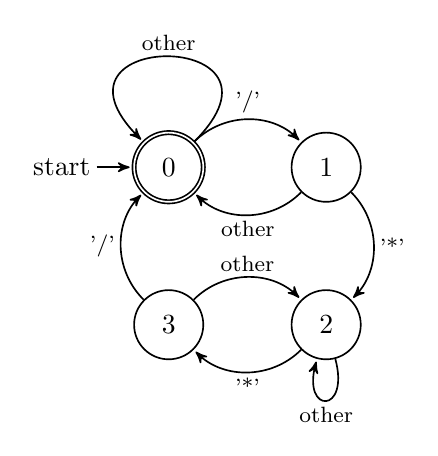
\begin{tikzpicture}[->, >=stealth', shorten >=1pt, auto, node distance=2cm, semithick, inner sep=2pt, bend angle=45]
\node[initial, accepting, state] (s0) {0};
\node[state] (s1) [right of=s0] {1};
\node[state] (s2) [below of=s1] {2};
\node[state] (s3) [below of=s0] {3};
\tikzstyle{every node}=[font=\footnotesize]
\path 
(s0) edge [bend left] node {'/'} (s1)
(s0) edge [loop, above] node {other} (s0)

(s1) edge [bend left] node {other} (s0)
(s1) edge [bend left] node {'*'} (s2)

(s2) edge [bend left] node {'*'} (s3)
(s2) edge [loop below] node {other} (s2)

(s3) edge [bend left] node {'/'} (s0)
(s3) edge [bend left] node {other} (s2);
\end{tikzpicture}
\end{center}
\caption{消除注释}
\label{fig:comment}
\end{figure}

\subsubsection{突出引导符}

即是给引导符前后添加空格,保证fscanf读入时,能够单独读入引导符。本例中的引导符有三个:\&\&、$||$、$=>$。见图\ref{fig:ruleintro}。

\begin{figure}
\begin{center}
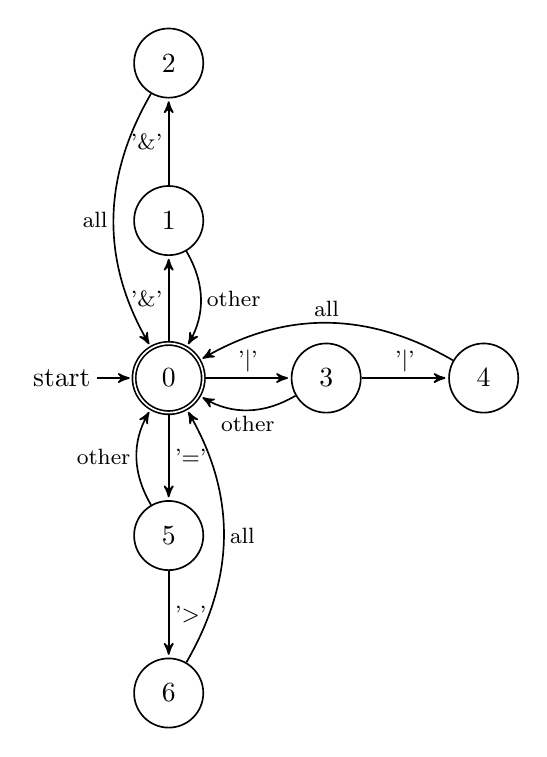
\begin{tikzpicture}[->, >=stealth', shorten >=1pt, auto, node distance=2cm, semithick, inner sep=2pt, bend angle=30]
\node[initial, accepting, state] (s0) {0};
\node[state] (s1) [above of=s0] {1};
\node[state] (s2) [above of=s1] {2};
\node[state] (s3) [right of=s0] {3};
\node[state] (s4) [right of=s3] {4};
\node[state] (s5) [below of=s0] {5};
\node[state] (s6) [below of=s5] {6};

\tikzstyle{every node}=[font=\footnotesize]
\path 
(s0) edge node {'\&'} (s1)
(s1) edge node {'\&'} (s2)

(s0) edge node {'$|$'} (s3)
(s3) edge node {'$|$'} (s4)

(s0) edge node {'$=$'} (s5)
(s5) edge node {'$>$'} (s6)

(s1) edge [bend left] node {other} (s0)
(s2) edge [bend right] node [left] {all} (s0)

(s3) edge [bend left] node {other} (s0)
(s4) edge [bend right] node [above] {all} (s0)

(s5) edge [bend left] node {other} (s0)
(s6) edge [bend right] node [right] {all} (s0);
\end{tikzpicture}
\end{center}
\caption{fig:ruleintro}
\end{figure}

\subsubsection{消除title}

见图\ref{fig:ruletitle}。

\begin{figure}
\begin{center}
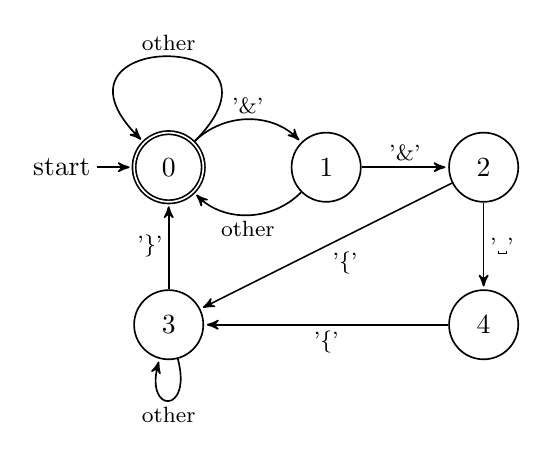
\begin{tikzpicture}[->, >=stealth', shorten >=1pt, auto, node distance=2cm, semithick, inner sep=2pt, bend angle=45]
\node[initial, accepting, state] (s0) {0};
\node[state] (s1) [right of=s0] {1};
\node[state] (s2) [right of=s1] {2};
\node[state] (s3) [below of=s0] {3};
\node[state] (s4) [below of=s2] {4};
\tikzstyle{every node}=[font=\footnotesize]
\path 
(s0) edge [bend left] node {'\&'} (s1)
(s0) edge [loop, above] node {other} (s0)

(s1) edge node {'\&'} (s2)
(s1) edge [bend left] node {other} (s0)

(s2) edge node {'\textvisiblespace'} (s4)
(s2) edge node {'\{'} (s3)

(s3) edge node {'\}'} (s0)
(s3) edge [loop below] node {other} (s3)

(s4) edge node {'\{'} (s3);
\end{tikzpicture}
\end{center}
\caption{消除title}
\label{fig:ruletitle}
\end{figure}

\subsection{浅层分析}

前面三个处理可以视为这个浅层分析的词法分析。因此,词法分析可以分解成多个方面的单独处理,即多次扫描完成。

\begin{center}
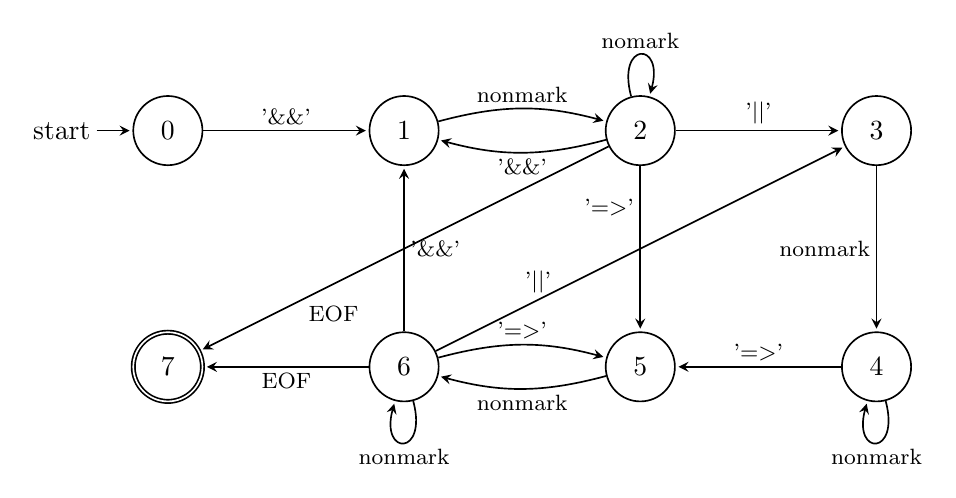
\begin{tikzpicture}[->, >=stealth, shorten >=1pt, auto, node distance=3cm, semithick, inner sep=2pt, bend angle=15]

\node[initial, state] (s0) {0};
\node[state] (s1) [right of=s0] {1};
\node[state] (s2) [right of=s1] {2};
\node[state] (s3) [right of=s2] {3};
\node[state] (s4) [below of=s3] {4};
\node[state] (s5) [left of=s4] {5};
\node[state] (s6) [left of=s5] {6};
\node[accepting, state] (s7) [left of=s6] {7};

\tikzstyle{every node}=[font=\footnotesize]
\path 
(s0) edge [above] node {'\&\&'} (s1)

(s1) edge [bend left] node {nonmark} (s2)

(s2) edge [bend left] node {'\&\&'} (s1)
(s2) edge [above] node {'$||$'} (s3)
(s2) edge [left, near start] node {'$=>$'} (s5)
(s2) edge [loop above] node {nomark} (s2)
(s2) edge [near end] node {EOF} (s7)

(s3) edge [left] node {nonmark} (s4)

(s4) edge [above] node {'$=>$'} (s5)
(s4) edge [loop below] node {nonmark} (s4)

(s5) edge [bend left] node {nonmark} (s6)

(s6) edge [right] node {'\&\&'} (s1)
(s6) edge [above, near start] node {'$||$'} (s3)
(s6) edge [bend left] node {'$=>$'} (s5)
(s6) edge [loop below] node {nonmark} (s6)
(s6) edge node {EOF} (s7);
\end{tikzpicture}

\vspace{0.5pc}
shallow() at file shallow.cc
\end{center}

其中用到三个引导符(也称标记字符串):“\&\&”、“$||$”、“$=>$”。图中nonmark表示其他字符串。这个分析的主要目的是将规则中的三大部分(短语结构规则、开关规则、转换规则)区分出来,并且给出这三部分的关系。即如下的一个树结构(图\ref{fig:rulerela}):

\begin{figure}
\begin{center}
  \begin{tikzpicture}[level/.style={sibling distance=30mm/#1}]
    \node [rectangle, draw] (prs) {短语结构规则}
    child { node [rectangle, draw] (swi1) {开关规则} 
      child { node [rectangle, draw] (trn11) {转换规则} }
      child { node (trn12) {...} }
      child { node [rectangle, draw] (trn13) {转换规则} }
    } 
    child { node (swi2) {...} }
    child { node [rectangle, draw] (swi3) {开关规则} 
      child { node [rectangle, draw] (trn31) {转换规则} }
      child { node (trn32) {...} }
      child { node [rectangle, draw] (trn33) {转换规则} }
    };
  \end{tikzpicture}
\end{center}
\caption{规则中各部分的关系}
\label{fig:rulerela}
\end{figure}

即一个短语结构规则可以有多个开关规则,一个开关规则可以有多个转换规则。另外,规则中允许出现如下的简略形式:
\begin{itemize*}
\item 没有开关规则和转换规则
\item 没有开关规则,只有转换规则
\end{itemize*}
但是不允许出现:有开关规则,没有转换规则。对于这些简略形式,我们引入空规则来表示,即开关规则和转换规则可以为空,但是有一个条件限制:即不能出现开关规则为空,而转换规则不为空。

下面说明,如何沿着状态图转移中,构造这样的树。分状态讨论,当程序进入该状态时,应做如下处理:
\begin{itemize*}
\item 状态1:当前token一定是非引导符,是一个短语结构规则的开始,记录在prs中;
\item 状态2:根据当前token的值,分四种情况讨论(token的值只可能是这四中情况中的一种):
\begin{itemize*}
\item 为nonmark:是一个短语结构的一部分,顺序记录在prs中;
\item 为\&\&:是短语结果规则的引导符,不处理;
\item 为$||$:是开关规则的引导符,不处理;
\item 为$=>$:是转换规则的引导符,说明当前的开关规则为空,令swi=空。
\end{itemize*}
\item 状态3:当前token一定是非引导符,是一个开关规则的开始,记录在swi中;
\item 状态4:当前token可能出现两种情况,分别讨论如下:
\begin{itemize*}
\item 为nonmark:是开关规则的一部分,顺序记录在swi中;
\item 为$=>$:是转换规则的引导符,不处理。
\end{itemize*}
\item 状态5:当前token一定是非引导符,是一个转换规则的开始,记录在tran中。
\item 状态6:类似状态2,分四种情况讨论:
\begin{itemize*}
\item 为nonmark:是一个转换规则的一部分,顺序记录在tran中;
\item 为\&\&:是短语结果规则的引导符,不处理;
\item 为$||$:是开关规则的引导符,不处理;
\item 为$=>$:是转换规则的引导符,说明当前的开关规则为空,令swi=空。
\end{itemize*}
\end{itemize*}

上面的状态转移和处理还可以总结在一张表(Action Table)中:

\vspace{1pc}
\begin{tabular}{|p{0.05\textwidth}|p{0.15\textwidth}|p{0.15\textwidth}|p{0.15\textwidth}|p{0.15\textwidth}|p{0.15\textwidth}|}
\hline
状态 & \&\& & $||$ & $=>$ & nonmark & EOF \\
\hline
0 & 1 & error & error & error & error \\
\hline
1 & error & error & error & 
\begin{tabular}{@{}l}
2 \\
prs = curstr
\end{tabular} 
& error \\
\hline
2 & 
\begin{tabular}{@{}l}
1 \\
当前规则结束,\\
保存进ruleset。\\
prs, switranset
\end{tabular}
& 3 & 5 & 
\begin{tabular}{@{}l}
2 \\
prs += curstr
\end{tabular} 
&
\begin{tabular}{@{}l}
1 \\
当前规则结束,\\
保存进ruleset。\\
prs, switranset
\end{tabular} \\
\hline
3 & error & error & error & 
\begin{tabular}{@{}l}
4 \\
swi = curstr
\end{tabular} 
& error \\
\hline
4 & error & error & 5 & 
\begin{tabular}{@{}l}
4 \\
swi += curstr
\end{tabular} 
& error \\
\hline
5 & error & error & error & 
\begin{tabular}{@{}l}
6 \\
tran = curstr
\end{tabular} 
& error
\\
\hline
6 & 
\begin{tabular}{@{}l}
1 \\
当前规则结束,\\
保存进ruleset。\\
prs, switranset
\end{tabular}
& 
\begin{tabular}{@{}l}
3 \\
当前switran结束,\\
保存进switranset。\\
swi, transet
\end{tabular}
& 
\begin{tabular}{@{}l}
5 \\
当前tran结束,\\
保存进transet。\\
tran
\end{tabular}
& 
\begin{tabular}{@{}l}
6 \\
tran += curstr 
\end{tabular}
&
\begin{tabular}{@{}l}
1 \\
当前规则结束,\\
保存进ruleset。\\
prs, switranset
\end{tabular}
\\
\hline
\end{tabular}

\vspace{1pc}
将上面的表转换成程序,如下:

\begin{verbatim}
switch (state) {
  0: 
  switch (curstr) {
    \&\&: state=1;break;
    other: error();
  }
  break;
  1:
  switch (curstr) {
    nonmark: state=2; prs=curstr; break;
    other: error();
  }
  break;
  2:
  switch (curstr) {
    \&\&: state=1; saveprs(); break;
    $||$: state=3; saveprs(); break;
    $=>$: state=5; saveprs(); break; 
    other: state=2; prs += curstr;
  }
  break;
  3:
  switch (curstr) {
    nonmark: state=4; swi=curstr; break;
    other: error();
  }
  break;
  4:
  switch (curstr) {
    $=>$: state=5; saveswi(); break;
    nonmark: state=4; swi+=curstr; break;
    other: error();
  }
  break;
  5:
  switch (curstr) {
    nonmark: state=6; tran=curstr; break;
    other: error();
  }
  break;
  6:
  switch (curstr) {
    \&\&: state=1; savetran(); break;
    $||$: state=3; savetran(); break;
    $=>$: state=5; savetran(); break;
    other: state=6; tran+=curstr;
  }
}
\end{verbatim}

下面讨论上面的三个保存函数。

\begin{verbatim}
class switranclass {
  puclic:
  string swi;
  set<string> transet;
}

class ruleclass {
  public:
  string prs;
  set<switranclass> switranset;
}

void savetran()
{
  transet.insert(tran);
}

void saveswi()
{
  switranclass switran;
  switran.swi=swi;
  switran.transet=transet;
  switranset.insert(switran);
}

void saveprs()
{
  ruleclass rule;
  rule.prs=prs;
  rule.switranset=switranset;
  ruleset.insert(rule);
}
\end{verbatim}

本步具体实现参见函数shallow()(shallow.cc文件)。注意,处理完成后,字符串中不会出现两个或两个以上的空格。

\subsection{进一步分析}

上面的浅层分析完成后,我们知道了规则中的三个部分,内容保存在数据结构ruleset中。下面需要对这三个部分分别进一步分析,基本思路是:

\vspace{1pc}
\begin{verbatim}
for (set<ruleclass>::iterator i=ruleset.begin(); i!=ruleset.end(); i++) {
  分析i->prs;
  for (set<switranclass>::iterator j=i->switranset.begin(); j!=i->switranset.end(); j++) {
    分析j->swi;
    for (set<string>::iterator k=j->transet.begin(); k!=j->transet.end(); k++) {
      分析*k;
    }
  }
}
\end{verbatim}

\subsubsection{短语结构规则的分析}

短语结构规则的主要形式是:
\begin{verbatim}
<PrsStruct>:
        <PrsReductn> -> <PrsForest>
        <PrsReductn> -> <PrsForest> :: <PrsBind>
\end{verbatim}
因此主要有三个部分:\verb|<PrsReductn>|、\verb|<PrsForest>|和\verb|<PrsBind>|。与前面类似,利用两个引导符,产生式引导符“$->$”和约束引导符“::”,能够容易地完成这三部分的切分。现在将前面的prs类型从string改进为:
\begin{verbatim}
class prsclass {
  public:
  string reduct;
  string forest;
  string bind;
}
\end{verbatim}

\vspace{1pc}
\begin{center}
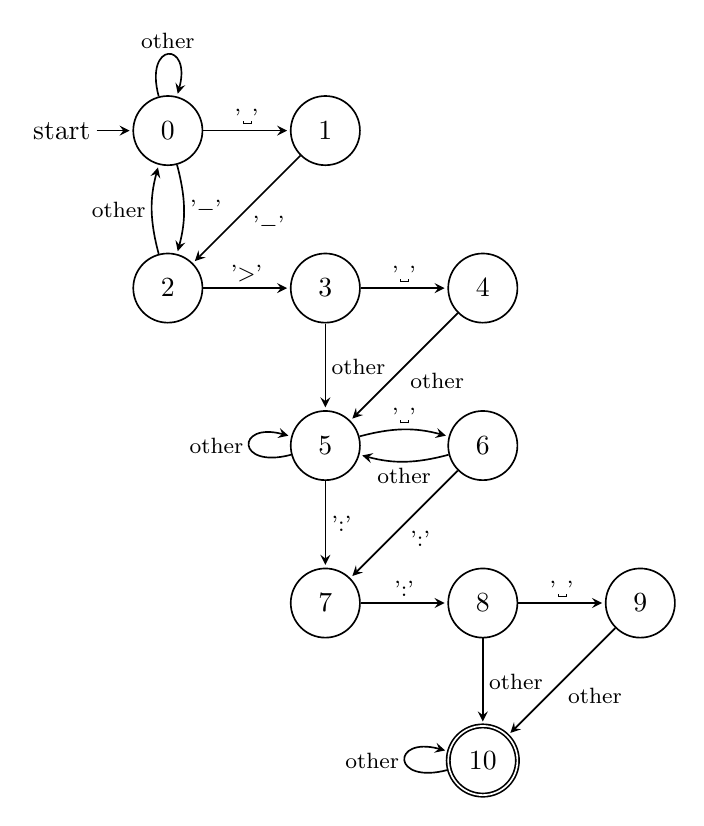
\begin{tikzpicture}[->, >=stealth, shorten >=1pt, auto, node distance=2cm, semithick, inner sep=2pt, bend angle=15]

\node[initial, state] (s0) {0};
\node[state] (s1) [right of=s0] {1};
\node[state] (s2) [below of=s0] {2};
\node[state] (s3) [right of=s2] {3};
\node[state] (s4) [right of=s3] {4};
\node[state] (s5) [below of=s3] {5};
\node[state] (s6) [right of=s5] {6};
\node[state] (s7) [below of=s5] {7};
\node[state] (s8) [right of=s7] {8};
\node[state] (s9) [right of=s8] {9};
\node[accepting, state] (s10) [below of=s8] {10};

\tikzstyle{every node}=[font=\footnotesize]
\path 
(s0) edge [loop above] node {other} (s0)
(s0) edge node {'\textvisiblespace'} (s1)
(s0) edge [bend left] node {'$-$'} (s2)

(s1) edge node {'$-$'} (s2)

(s2) edge node {'$>$'} (s3)
(s2) edge [bend left] node {other} (s0)

(s3) edge node {'\textvisiblespace'} (s4)
(s3) edge node {other} (s5)

(s4) edge node {other} (s5)

(s5) edge [loop left] node {other} (s5)
(s5) edge [bend left] node {'\textvisiblespace'} (s6)
(s5) edge node {':'} (s7)

(s6) edge [bend left] node {other} (s5)
(s6) edge node {':'} (s7)

(s7) edge node {':'} (s8)

(s8) edge node {'\textvisiblespace'} (s9)
(s8) edge node {other} (s10)

(s9) edge node {other} (s10)

(s10) edge [loop left] node {other} (s10);

\end{tikzpicture}

\vspace{0.5pc}
shallow2() at file shallow.cc
\end{center}

三个部分中,\verb|<PrsReductn>|很简单,下面重点讨论\verb|<PrsForest>|和\verb|<PrsBind>|的进一步分析。查看文法(参见附录)得到,
\begin{verbatim}
<PrsForest>:
        <LeftForest>
        ^ <LeftForest>
<LeftForest>:
        <LeftTree>
        <HeadTag> <LeftTree>
        <LeftForest> <LeftForest>
<LeftTree>:
        <LabelItem>
        <LabelItem> < <WordItem_Or> >
        <LabelItem> ( <LeftSubForest> )
<LeftSubForest>:
        <LeftSubTree>
        <HeadTag> <LeftSubTree>
        <LeftSubForest> <LeftSubForest>
<LeftSubTree>:
        <LeftLabelItem>
        <LeftLabelItem> < <WordItem_Or> >
        <LeftLabelItem> ( <LeftSubForest> )
<LeftLabelItem>:
        <LabelItem>
<LabelItem>:
        <Ident:LexCat>
        <Ident:PhrCat>
<WordItem_Or>:
        <WordItem>
        <WordItem_Or> | <WordItem>
<WordItem>:
        ~~
        <Word>
<Word>:
        <Ident>
<HeadTag>:
        !
\end{verbatim}

这一段文法比前面要复杂很多,似乎只有使用LR分析法了。但是我们继续避免用一般的LR方法,我们认为那种方法是机器对文法没有很好理解的情况下的一种低效的方法。首先,我们再次发现两组特殊的符号$<,>$和$()$。我们先将它们分析出来。

\vspace{1pc}
\begin{center}
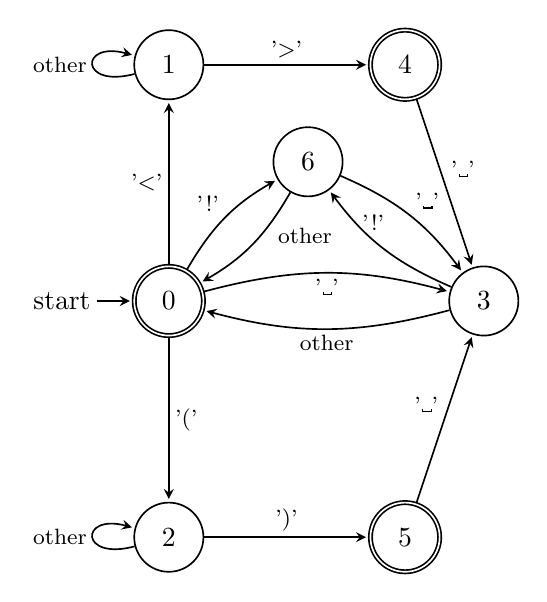
\begin{tikzpicture}[->, >=stealth, shorten >=1pt, auto, node distance=4cm, semithick, inner sep=2pt, bend angle=15]

\node[initial, accepting, state] (s0) {0};
\node[state] (s1) [node distance=3cm, above of=s0] {1};
\node[state] (s2) [node distance=3cm, below of=s0] {2};
\node[state] (s3) [right of=s0] {3};
\node[accepting, state] (s4) [node distance=3cm, right of=s1] {4};
\node[accepting, state] (s5) [node distance=3cm, right of=s2] {5};
\node[state] (s6) [node distance=2.5cm, above right of=s0] {6};

\tikzstyle{every node}=[font=\footnotesize]
\path 
(s0) edge node {'$<$'} (s1)
(s0) edge node {'('} (s2)
(s0) edge [below, bend left] node {'\textvisiblespace'} (s3)
(s0) edge [bend left] node {'!'} (s6)

(s1) edge [loop left] node {other} (s1)
(s1) edge node {'$>$'} (s4)

(s2) edge [loop left] node {other} (s2)
(s2) edge node {')'} (s5)

(s3) edge [near end, right, bend left] node {'!'} (s6)
(s3) edge [bend left] node {other} (s0)

(s4) edge node {'\textvisiblespace'} (s3)

(s5) edge node {'\textvisiblespace'} (s3)

(s6) edge [bend left] node {'\textvisiblespace'} (s3)
(s6) edge [near start, bend left] node {other} (s0);

\end{tikzpicture}

\vspace{0.5pc}
shallow3() at file shallow.cc
\end{center}

\vspace{1pc}
再看有关\verb|<PrsBind>|的文法。

\begin{verbatim}
<PrsBind>:
        <Bind>
<Bind>:
        <Equation>
        <Test>
        <Bind> , <Bind>
<Test>:
        IF <Bind> TRUE
        IF <Bind> FALSE
        IF <Bind> THEN <Bind> ENDIF
        IF <Bind> ELSE <Bind> ENDIF
        IF <Bind> THEN <Bind> ELSE <Bind> ENDIF
<Equation>:
        <IntVar> = <Atom>
        <IntVar> = <IntVar>
        <ExtVar> = <Fest>
        <ExtVar> = <ExtVar>
        <ExtVar> = <True>
        <ExtVar> = <False>
        <ExtVar> == <ExtVar> <At>
        <ExtVar> != <ExtVar> <At>
<ExtVar>:
        <RootVar>
        <LabelVar>
        <ExtVar>.<ExtAtt>
<IntVar>:
        <ExtVar>.<IntAtt>
<RootVar>:
        $
<At>:
        @ <Ident:IntAtt>
        @ <Ident:ExtAtt>
        <At> <At>
\end{verbatim}

\vspace{1pc}
可见\verb|<PrsBind>|就是\verb|<Bind>|。由多个组成,用逗号“,”分开。\verb|<Bind>|有两种形式:类似等式的形式和带有IF的形式。其中,带有IF的形式比较复杂,其中可以再次嵌入\verb|<Bind>|的形式。前一种形式可以视为后一种的特例,因此我们可以将所有的形式写成如下的形式:

\verb|IF <Bind> THEN <Bind> ELSE <Bind> ENDIF|

其对应关系如下表。

\begin{verbatim}
<Equation>
IF TRUE THEN <Equation> ELSE NULL ENDIF

IF <Bind> TRUE
IF <Bind> THEN TRUE ELSE NULL ENDIF (或者)
IF <Bind> THEN TRUE ELSE FALSE ENDIF

IF <Bind> FALSE
IF <Bind> THEN FALSE ELSE NULL ENDIF (或者)
IF <Bind> THEN FALSE ELSE TRUE ENDIF

IF <Bind> THEN <Bind> ENDIF
IF <Bind> THEN <Bind> ELSE NULL ENDIF

IF <Bind> ELSE <Bind> ENDIF
IF <Bind> THEN NULL ELSE <Bind> ENDIF
\end{verbatim}

\vspace{1pc}
第一步先预处理,给每个分隔符“,”左右添加空格。我们先处理IF的形式。其FA如下:

\vspace{1pc}
\begin{center}
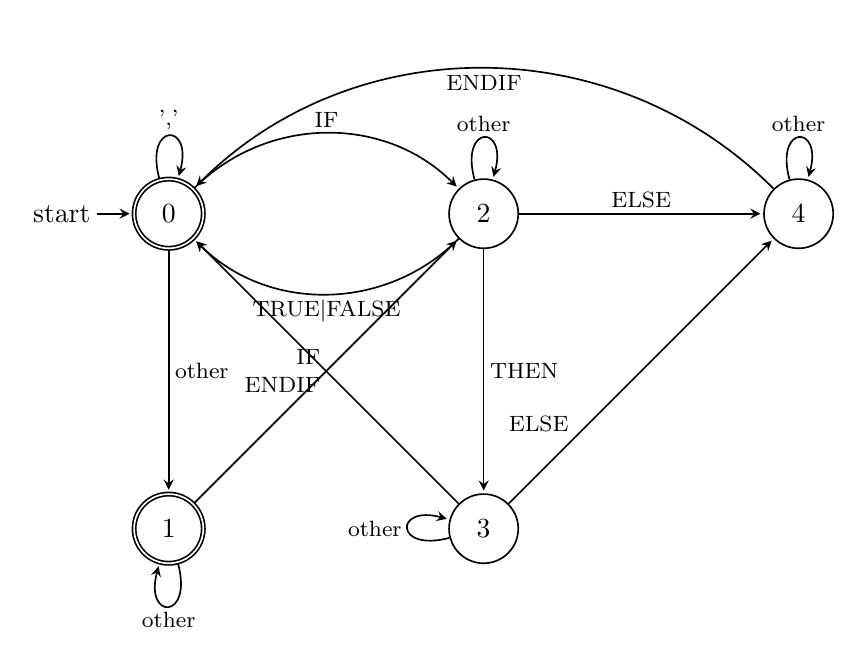
\begin{tikzpicture}[->, >=stealth, shorten >=1pt, auto, node distance=4cm, semithick, inner sep=2pt, bend angle=45]

\node [initial, accepting, state] (s0) {0};
\node [accepting, state] (s1) [below of=s0] {1};
\node [state] (s2) [right of=s0] {2};
\node [state] (s3) [below of=s2] {3};
\node [state] (s4) [right of=s2] {4};

\tikzstyle{every node}=[font=\footnotesize]
\path 
(s0) edge [loop above] node {','} (s0)
(s0) edge [bend left] node {IF} (s2)
(s0) edge node {other} (s1)

(s1) edge [loop below] node {other} (s1)
(s1) edge node {IF} (s2)

(s2) edge [bend left] node {TRUE$|$FALSE} (s0)
(s2) edge [right] node {THEN} (s3)
(s2) edge node {ELSE} (s4)
(s2) edge [loop above] node {other} (s2)

(s3) edge [near start] node {ELSE} (s4)
(s3) edge node {ENDIF} (s0)
(s3) edge [loop left] node {other} (s3)

(s4) edge [bend right, bend angle=45] node {ENDIF} (s0)
(s4) edge [loop above] node {other} (s4);
\end{tikzpicture}
\end{center}

处理约束部分的FA如下。

\vspace{1pc}
\begin{center}
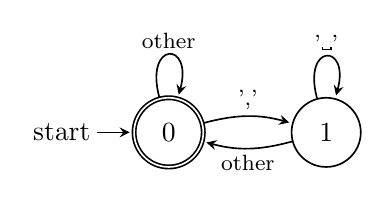
\begin{tikzpicture}[->, >=stealth, shorten >=1pt, auto, node distance=2cm, semithick, inner sep=2pt, bend angle=15]

\node [initial, accepting, state] (s0) {0};
\node [state] (s1) [right of=s0] {1};

\tikzstyle{every node}=[font=\footnotesize]
\path 
(s0) edge [bend left] node {','} (s1)
(s0) edge [loop above] node {other} (s0)
(s1) edge [loop above] node {'\textvisiblespace'} (s1)
(s1) edge [bend left] node {other} (s0);
\end{tikzpicture}
\end{center}

\subsubsection{转换规则的分析}

先看它的文法,

\vspace{1pc}
\begin{verbatim}
<TrnStruct>:
        <TrnTree>
        <TrnTree> <TrnBind>
<TrnTree>:
        <RightTree>
<TrnBind>:
        <Bind>
<RightTree>:
        <LabelItem>
        <LabelItem> < <WordItem_Or> >
        <LabelItem> ( <RightSubForest> )
<RightSubForest>:
        <RightSubTree>
        <HeadTag> <RightSubTree>
        <MoveTag> <ShiftLabelItem>
        <RemvTag> <ShiftLabelItem>
        <CopyTag> <ShiftLabelItem>
        <SubForest> <RightSubForest>
<RightSubTree>:
        <RightLabelItem>
        <RightLabelItem> < <WordItem_Or> >
        <RightLabelItem> ( <RightSubForest> )
<RightLabelItem>:
        <LabelItem>
        <LabelItem> <TransVar>
<ShiftLabelItem>:
        <LabelItem> <LabelVar>
\end{verbatim}

\vspace{1pc}
分析其中的规律,得到如下结论:
\begin{itemize*}
\item \verb|<TrnStruct>|由两部分组成:\verb|<TrnTree>|和\verb|<TrnBind>|。其中
\item \verb|<TrnTree>|有三种形式,
\item \verb|<TrnBind>|与前面的\verb|<Bind>|文法相同。
\end{itemize*}
分析过程如下:先将这两个部分切分开,然后各自独立分析。

\vspace{1pc}
\begin{center}
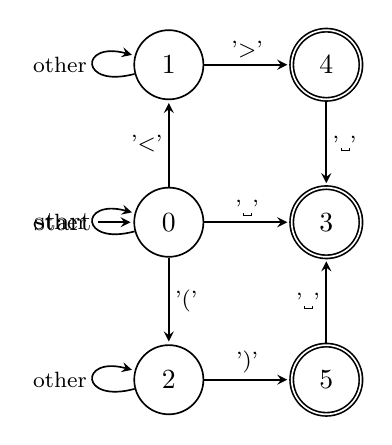
\begin{tikzpicture}[->, >=stealth, shorten >=1pt, auto, node distance=2cm, semithick, inner sep=2pt, bend angle=15]
\node [initial, state] (s0) {0};
\node [state] (s1) [above of=s0] {1};
\node [state] (s2) [below of=s0] {2};
\node [accepting, state] (s3) [right of=s0] {3};
\node [accepting, state] (s4) [right of=s1] {4};
\node [accepting, state] (s5) [right of=s2] {5};

\tikzstyle{every node}=[font=\footnotesize]
\path 
(s0) edge [loop left] node {other} (s0)
(s0) edge node {'$<$'} (s1)
(s0) edge node {'('} (s2)
(s0) edge node {'\textvisiblespace'} (s3)
(s1) edge [loop left] node {other} (s1)
(s1) edge node {'$>$'} (s4)
(s2) edge [loop left] node {other} (s2)
(s2) edge node {')'} (s5)
(s4) edge node {'\textvisiblespace'} (s3)
(s5) edge node {'\textvisiblespace'} (s3);

\end{tikzpicture}
\end{center}

\subsubsection{转换规则中对应关系的分析}

有关短语对应关系的文法是,

\vspace{1pc}
\begin{verbatim}
<TransVar>:
        <TransVarTag> <LabelItem>
<TransVarTag>:
        /
        //
        ///
        ////
\end{verbatim}

我们设计如下的FA。

\vspace{1pc}
\begin{center}
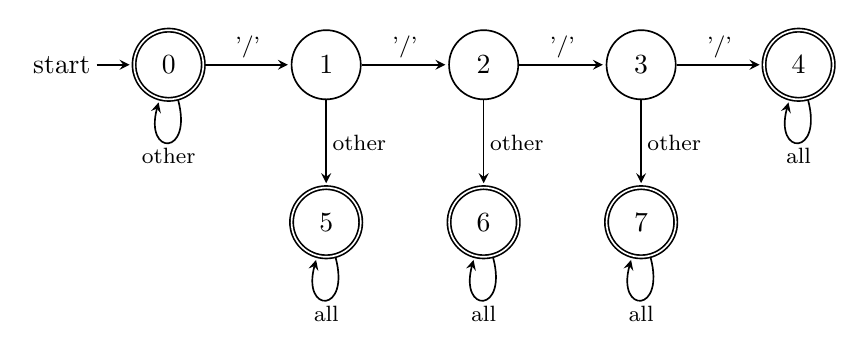
\begin{tikzpicture}[->, >=stealth, shorten >=1pt, auto, node distance=2cm, semithick, inner sep=2pt, bend angle=15]
\node [initial, accepting, state] (s0) {0};
\node [state] (s1) [right of=s0] {1};
\node [state] (s2) [right of=s1] {2};
\node [state] (s3) [right of=s2] {3};
\node [accepting, state] (s4) [right of=s3] {4};
\node [accepting, state] (s5) [below of=s1] {5};
\node [accepting, state] (s6) [below of=s2] {6};
\node [accepting, state] (s7) [below of=s3] {7};


\tikzstyle{every node}=[font=\footnotesize]
\path 
(s0) edge [loop below] node {other} (s0)
(s0) edge node {'/'} (s1)

(s1) edge node {'/'} (s2)
(s1) edge node {other} (s5)

(s2) edge node {'/'} (s3)
(s2) edge node {other} (s6)

(s3) edge node {'/'} (s4)
(s3) edge node {other} (s7)

(s4) edge [loop below] node {all} (s4)
(s5) edge [loop below] node {all} (s5)
(s6) edge [loop below] node {all} (s6)
(s7) edge [loop below] node {all} (s7);
\end{tikzpicture}
\end{center}

\subsubsection{将规则形式转换成平行的形式}

最后,我们将规则转换成对称的形式(或称平行形式),即不是以汉语为主,也不是以英语为主,其文法是:

\begin{verbatim}
<规则> : 
        <汉语规则> => <英语规则> <对应关系>
<汉语规则> :
        <短语规则>
<英语规则> :
        <短语规则>
<短语规则> :
        <产生式规则> <中心> <约束>
\end{verbatim}

一个规则的典型形式如下:
\begin{verbatim}
ap -> ap mp 0 :: 
    $.内部结构=组合述补,$.述语=%ap,$!=%ap @补语,$.补语=%mp, 
    IF %ap.内部结构=附加 THEN %ap.附加语.yx=了 ENDIF,
    %ap.内部结构=附加|述补,%mp.量词子类=~不定~动量, 
    IF %ap.内部结构=附加 THEN %ap.附加语.yx=了 ENDIF, 
    IF %ap.内部结构=述补,%ap.补语.内部结构=~单词 THEN %ap.补语.cpcat=~mp ENDIF
=>
AP -> AP P NP 0 :: 
    %1.yx=for
0 -1 1 
\end{verbatim}

\section{词典的分析}

前面讨论了规则的分析,下面说明词典的分析。其文法是,

\begin{verbatim}
<Entry>:
        $$ <Word> <Meaning>
        <Entry> <Meaning>
        <Entry> <PrsRule>
<Meaning>:
        ** { <Title> } <SrcMeaning>
        <Meaning> || <TrnSwitch> => <TgtMeaning>
        <Meaning> => <TgtMeaning>
<SrcMeaning>:
        <LabelItem>
        <LabelItem> <Bind>
<TgtMeaning>:
        <TrnStruct>
<TrnStruct>:
        <TrnTree>
        <TrnTree> <TrnBind>
\end{verbatim}

分析这个文法,词典由多个词条组成,一个典型的词条包括如下部分:

\begin{verbatim}
$$ <Word> ** { <Title> } <LabelItem> <Bind> || <TrnSwitch> => <TgtMeaning> <PrsRule>
\end{verbatim}

\begin{verbatim}
$$ <Word> ** { <Title> } <LabelItem> <Bind> || <TrnSwitch> => <TrnTree> <TrnBind> <PrsRule>
\end{verbatim}

其中 \verb|<Bind>|、\verb|<TrnSwitch>|、\verb|<TgtMeaning>|都可以省略。或者\verb|<TrnSwitch>|、\verb|<TgtMeaning>|可以出现多次,其关系类似规则中的表述(图\ref{fig:rulerela})。参见图\ref{fig:dictrela}。

\begin{figure}
  \begin{center}
    \begin{tikzpicture}[level/.style={sibling distance=30mm/#1}]
      \node [rectangle, draw] (word) {单词}
      child { node [rectangle, draw] (label) {词类,约束}
        child { node [rectangle, draw] (swi1) {开关规则} 
          child { node [rectangle, draw] (trn11) {译词} }
          child { node (trn12) {...} }
          child { node [rectangle, draw] (trn13) {译词} }
        } 
        child { node (swi2) {...} }
        child { node [rectangle, draw] (swi3) {开关规则} 
          child { node [rectangle, draw] (trn31) {译词} }
          child { node (trn32) {...} }
          child { node [rectangle, draw] (trn33) {译词} }
        }
      }
      child { node (label2) {...} };
    \end{tikzpicture}
  \end{center}
  \caption{规则中各部分的关系}
  \label{fig:dictrela}
\end{figure}

从语义上解释,其中
\begin{itemize*}
\item \verb|<Word>|是词语的原形(词语本身)
\item \verb|<LabelItem>|是词语的类别(词类)
\item \verb|<Bind>|是词语的属性集
\item \verb|<TrnSwitch>|是词语翻译的约束
\item \verb|<TrnTree>|是翻译的结果(一个词或者一个短语)
\item \verb|<TrnBind>|是对应译文的约束
\end{itemize*}

\subsection{预处理}

因此可以首先借助4个引导符\$\$、**、$||$、$=>$将这几部分分开。然后,再分别进一步分析。总的来说,词典的分析类似规则的分析,大致过程是:先预处理,然后浅层分析切分成几个大的部分,最后各个部分深入分析。其中,预处理与规则的分析相同,包括三个步骤:1)去除注释;2)突出引导符(即引导符前后加空格);3)去除title部分(title部分被视为文法中的无用信息)。其中,第一个步骤完全相同,后面两个步骤要相应修改(实际上,这两组程序可以合并,即实现一个通用的、统一的预处理程序)。结果如图\ref{fig:dictintro}所示。

\begin{figure}
\begin{center}
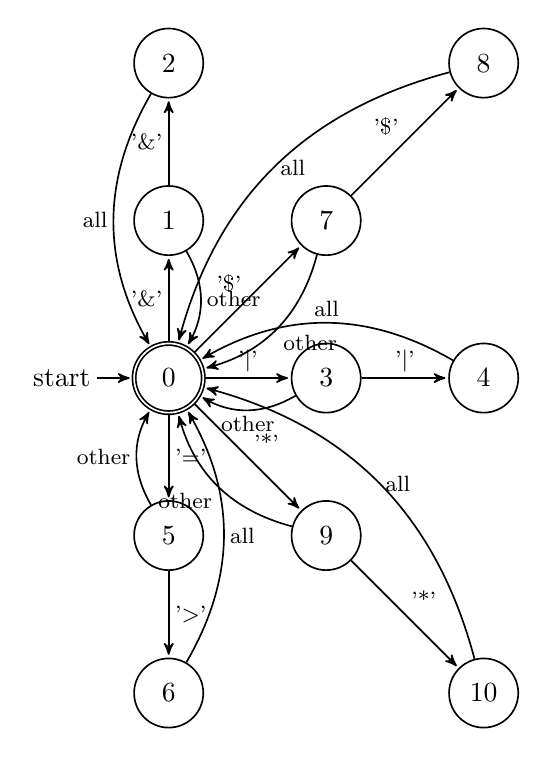
\begin{tikzpicture}[->, >=stealth', shorten >=1pt, auto, node distance=2cm, semithick, inner sep=2pt, bend angle=30]
\node[initial, accepting, state] (s0) {0};
\node[state] (s1) [above of=s0] {1};
\node[state] (s2) [above of=s1] {2};
\node[state] (s3) [right of=s0] {3};
\node[state] (s4) [right of=s3] {4};
\node[state] (s5) [below of=s0] {5};
\node[state] (s6) [below of=s5] {6};
\node[state] (s7) [right of=s1] {7};
\node[state] (s8) [node distance=4cm, right of=s2] {8};
\node[state] (s9) [right of=s5] {9};
\node[state] (s10) [node distance=4cm, right of=s6] {10};

\tikzstyle{every node}=[font=\footnotesize]
\path 
(s0) edge node {'\&'} (s1)
(s1) edge node {'\&'} (s2)

(s0) edge node {'$|$'} (s3)
(s3) edge node {'$|$'} (s4)

(s0) edge node {'$=$'} (s5)
(s5) edge node {'$>$'} (s6)

(s0) edge node {'\$'} (s7)
(s7) edge node {'\$'} (s8)

(s0) edge node {'*'} (s9)
(s9) edge node {'*'} (s10)

(s1) edge [bend left] node {other} (s0)
(s2) edge [bend right] node [left] {all} (s0)

(s3) edge [bend left] node {other} (s0)
(s4) edge [bend right] node [above] {all} (s0)

(s5) edge [bend left] node {other} (s0)
(s6) edge [bend right] node [right] {all} (s0)

(s7) edge [bend left] node {other} (s0)
(s8) edge [bend right] node [right] {all} (s0)

(s9) edge [bend left] node {other} (s0)
(s10) edge [bend right] node [right] {all} (s0);
\end{tikzpicture}
\end{center}
\caption{突出引导符}
\label{fig:dictintro}
\end{figure}

\begin{figure}
\begin{center}
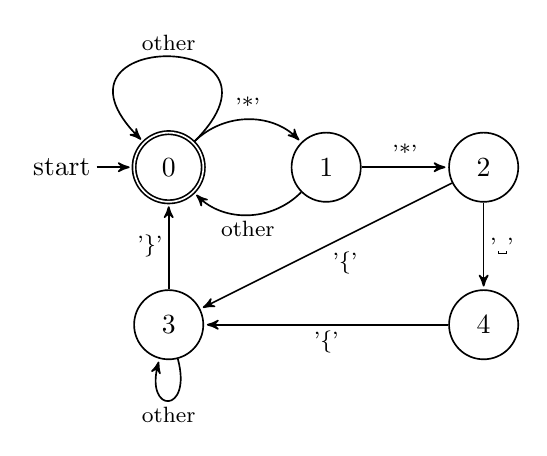
\begin{tikzpicture}[->, >=stealth', shorten >=1pt, auto, node distance=2cm, semithick, inner sep=2pt, bend angle=45]
\node[initial, accepting, state] (s0) {0};
\node[state] (s1) [right of=s0] {1};
\node[state] (s2) [right of=s1] {2};
\node[state] (s3) [below of=s0] {3};
\node[state] (s4) [below of=s2] {4};
\tikzstyle{every node}=[font=\footnotesize]
\path 
(s0) edge [bend left] node {'*'} (s1)
(s0) edge [loop, above] node {other} (s0)

(s1) edge node {'*'} (s2)
(s1) edge [bend left] node {other} (s0)

(s2) edge node {'\textvisiblespace'} (s4)
(s2) edge node {'\{'} (s3)

(s3) edge node {'\}'} (s0)
(s3) edge [loop below] node {other} (s3)

(s4) edge node {'\{'} (s3);
\end{tikzpicture}
\end{center}
\caption{消除title}
\label{fig:dicttitle}
\end{figure}

\subsection{浅层分析}

\begin{figure}
  \begin{center}
    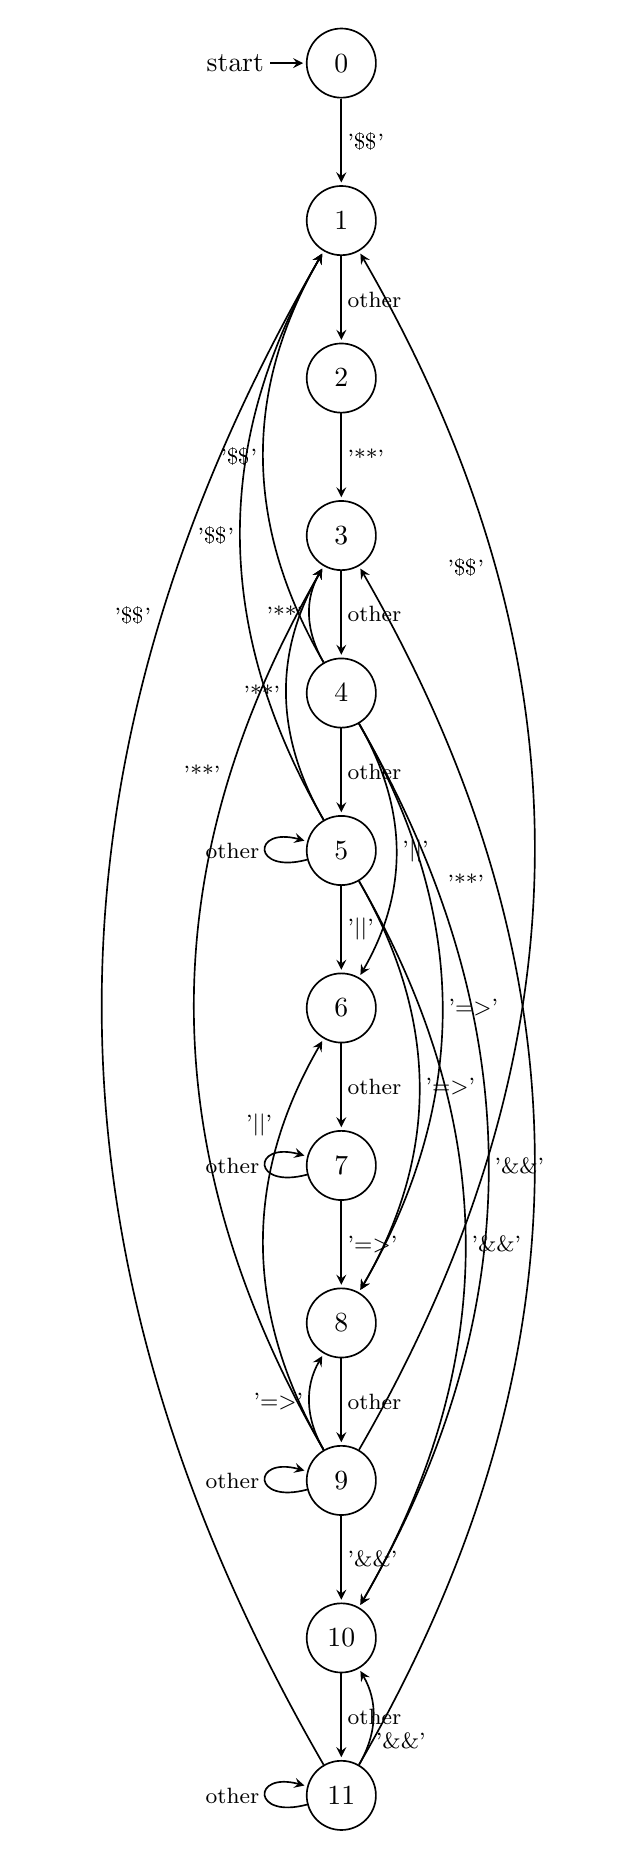
\begin{tikzpicture}[->, >=stealth, shorten >=1pt, auto, node distance=2cm, semithick, inner sep=2pt, bend angle=30]
      
      \node[initial, state] (s0) {0};
      \node[state] (s1) [below of=s0] {1};
      \node[state] (s2) [below of=s1] {2};
      \node[state] (s3) [below of=s2] {3};
      \node[state] (s4) [below of=s3] {4};
      \node[state] (s5) [below of=s4] {5};
      \node[state] (s6) [below of=s5] {6};
      \node[state] (s7) [below of=s6] {7};
      \node[state] (s8) [below of=s7] {8};
      \node[state] (s9) [below of=s8] {9};
      \node[state] (s10) [below of=s9] {10};
      \node[state] (s11) [below of=s10] {11};
      
      \tikzstyle{every node}=[font=\footnotesize]
      \path 
      (s0) edge node {'\$\$'} (s1)
      (s1) edge node {other} (s2)
      (s2) edge node {'**'} (s3)
      (s3) edge node {other} (s4)
      
      (s4) edge node {other} (s5)
      (s4) edge [bend left] node {'\$\$'} (s1)
      (s4) edge [bend left] node {'**'} (s3)
      (s4) edge [bend left] node {'$||$'} (s6)
      (s4) edge [bend left] node {'$=>$'} (s8)
      (s4) edge [bend left] node {'\&\&'} (s10)

      (s5) edge [loop left] node {other} (s5)
      (s5) edge [bend left] node {'\$\$'} (s1)
      (s5) edge [bend left] node {'**'} (s3)
      (s5) edge [bend left] node {'$=>$'} (s8)
      (s5) edge [bend left] node {'\&\&'} (s10)
      (s5) edge node {'$||$'} (s6)

      (s6) edge node {other} (s7)

      (s7) edge [loop left] node {other} (s7)
      (s7) edge node {'$=>$'} (s8)

      (s8) edge node {other} (s9)

      (s9) edge [loop left] node {other} (s9)
      (s9) edge [bend right] node [near end] {'\$\$'} (s1) 
      (s9) edge [bend left] node [near end] {'**'} (s3)
      (s9) edge [bend left, bend angle=45] node [near end] {'$||$'} (s6)
      (s9) edge [bend left] node {'$=>$'} (s8)
      (s9) edge node {'\&\&'} (s10)

      (s10) edge node {other} (s11)

      (s11) edge [loop left] node {other} (s11)
      (s11) edge [bend left] node [near end] {'\$\$'} (s1)
      (s11) edge [bend right, bend angle=45] node [near end] {'**'} (s3)
      (s11) edge [bend right] node [near start, right] {'\&\&'} (s10);
    \end{tikzpicture}
    \caption{词典的浅层分析(shallow() at file parsedict.cc)}
    \label{fig:dictshallow}
  \end{center}
\end{figure}

\section{规则、词典分析的合并}

我们看到词典中有大量规则出现(规则中没有出现词典信息),因此我们需要一个算法能够同时处理词典和规则。

\subsection{预处理的合并}

三个预处理,
\begin{itemize*}
\item 消除注释,两者是相同的。图\ref{fig:comment}。
\item 突出引导符,词典中的算法,即图\ref{fig:dictintro},已经合并了两者。
\item 消除title。需要合并图\ref{fig:ruletitle}和\ref{fig:dicttitle},结果如图\ref{fig:title}所示。
\end{itemize*}

\begin{figure}
\begin{center}
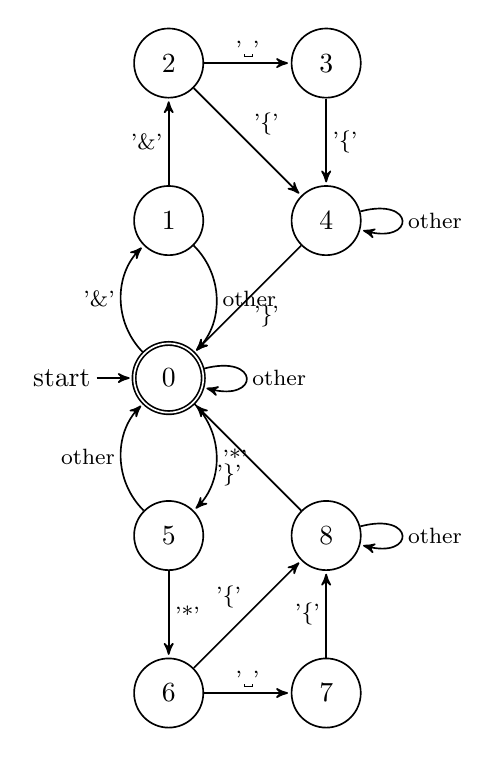
\begin{tikzpicture}[->, >=stealth', shorten >=1pt, auto, node distance=2cm, semithick, inner sep=2pt, bend angle=45]
\node[initial, accepting, state] (s0) {0};
\node[state] (s1) [above of=s0] {1};
\node[state] (s2) [above of=s1] {2};
\node[state] (s3) [right of=s2] {3};
\node[state] (s4) [below of=s3] {4};
\node[state] (s5) [below of=s0] {5};
\node[state] (s6) [below of=s5] {6};
\node[state] (s7) [right of=s6] {7};
\node[state] (s8) [above of=s7] {8};

\tikzstyle{every node}=[font=\footnotesize]
\path 
(s0) edge [loop right] node {other} (s0)
(s0) edge [bend left] node {'\&'} (s1)
(s0) edge [bend left] node {'*'} (s5)

(s1) edge [bend left] node {other} (s0)
(s1) edge node {'\&'} (s2)

(s2) edge node {'\textvisiblespace'} (s3)
(s2) edge node {'\{'} (s4)

(s3) edge node {'\{'} (s4)

(s4) edge node {'\}'} (s0)
(s4) edge [loop right] node {other} (s4)

(s5) edge [bend left] node {other} (s0)
(s5) edge node {'*'} (s6)

(s6) edge node {'\textvisiblespace'} (s7)
(s6) edge node {'\{'} (s8)

(s7) edge node {'\{'} (s8)

(s8) edge node {'\}'} (s0)
(s8) edge [loop right] node {other} (s8);
\end{tikzpicture}
\end{center}
\caption{消除title}
\label{fig:title}
\end{figure}

图\ref{fig:title}上下两部分对称,我们采用一种带参数的自动机状态图。如图\ref{fig:titlepara}所示。

\begin{figure}
\begin{center}
\begin{tikzpicture}[->, >=stealth', shorten >=1pt, auto, node distance=2cm, semithick, inner sep=2pt, bend angle=45]
\node[initial, accepting, state] (s0) {0};
\node[state] (s1) [above of=s0] {1:c};
\node[state] (s2) [above of=s1] {2:c};
\node[state] (s3) [right of=s2] {3:c};
\node[state] (s4) [below of=s3] {4:c};

\tikzstyle{every node}=[font=\footnotesize]
\path 
(s0) edge [loop right] node {other} (s0)
(s0) edge [bend left] node {'\&'或'*'} (s1)

(s1) edge [bend left] node {other} (s0)
(s1) edge node {输入与c相等} (s2)

(s2) edge node {'\textvisiblespace'} (s3)
(s2) edge node {'\{'} (s4)

(s3) edge [loop above] node {'\textvisiblespace'} (s3)
(s3) edge node {'\{'} (s4)

(s4) edge node {'\}'} (s0)
(s4) edge [loop right] node {other} (s4);
\end{tikzpicture}
\end{center}
\caption{消除title,带参数的自动机。每个状态有一个参数c。比如状态1的参数c记录导致转移到状态1的字符。状态2的c从1传递得到。详细说明看程序。}
\label{fig:title}
\end{figure}

\subsection{分析的合并}

主要工作是将规则分析中的函数模块化,并提供给词典分析的函数使用。

\section{中文分词的设计}

基于词典(和规则)的分词方法。首先,定义句子的数据结构是,

\begin{verbatim}
class wenziclass {
  public:
  string c;
};

vector<wenziclass> sentence;
\end{verbatim}

对于英文而言,其中的$c$是一个字节的字符串,中文utf8编码而言,主要是2字节的字符串,对于一些特殊的汉字,则可能是3字节或4字节。分词算法如下(这是一个典型的Viterbi算法):

\begin{verbatim}
/* 搜索部分 */
for (int i=0; i<=sentence.size(); i++) {
  /* 完成sentence[0,i]的切分; */
  for (int j=0; j<i; j++) {
    if (sentence[j,i]是一个词) {
      当前词个数=wordcount[j]+1;
    }
    /* 修正wordcount[j] */
    if (当前词个数 < wordcount[i]) {
      traceback[i]=j;
      wordcount[i]=当前词个数;
    }
  }
}

/* 回溯部分 */
for (int i=sentence.size(); i>0; i=traceback[i]) {
  segment[traceback[i]]=i;
}
\end{verbatim}

算法的思路是逐个扫描字间空隙(不是字本身,因此如果句子有$n$个字,那么扫描长度为$n+1$。),再向前判断切分的位置。这个算法的原始思想是一种递归的思想:

对于所有$0 \le i\le sentence.size()$,有
\begin{equation}
seg(0,i)=\text{best of} \left\{
\begin{array}{l}
  seg(0,i-1)+word(i-1,i); \\
  seg(0,i-2)+word(i-2,i); \\
  \ldots \\
  seg(0,j)+word(j,i); \\
  \ldots \\
  seg(0,1) + word(1,i);
\end{array}
\right. \label{equ:segword}
\end{equation}

上式有两点要说明:
\begin{itemize*}
\item 要求位置$j$到$i$形成词;
\item 前面的分词结果,即seg(0,j),是最优的。最简单的做法是认为其中的单词个数最少的切分是最优的。特别注意,上面的算法不能保证最后发现的结果是最优结果(可以举例说明)。但是容易发现多数情况下是最优结果,即使不是最优,也是非常接近最优的结果。
\end{itemize*}

当然更好的方法(但是时间复杂度更高)是,
\begin{equation}
seg(0,i)=\text{best of} \left\{
\begin{array}{l}
  seg(0,i-1)+seg(i-1,i); \\
  seg(0,i-2)+seg(i-2,i); \\
  \ldots \\
  seg(0,j)+seg(j,i); \\
  \ldots \\
  seg(0,1) + seg(1,i);
\end{array}
\right. \label{equ:segseg}
\end{equation}

可以想办法尝试证明这两个式子是等价的。

\section{句法分析}

下面我们尝试将分词的方法推广到句法分析。借用式子(\ref{equ:segword}),得到
\begin{equation}
seg(0,i)=\text{best of} \left\{
\begin{array}{l}
  parse(0,i-1)+phrase(i-1,i); \\
  parse(0,i-2)+phrase(i-2,i); \\
  \ldots \\
  parse(0,j)+phrase(j,i); \\
  \ldots \\
  parse(0,1) + phrase(1,i);
\end{array}
\right. \label{equ:parsephrase}
\end{equation}
即要完成两个条件:
\begin{itemize*}
\item 句子中的词语子串(j,i)要形成一个短语
\item (0,j)的分析结果与短语(j,i)结合形成的结果最优。
\end{itemize*}

当然,类似分词,更复杂的形式是如下,此处不做深入讨论。
\begin{equation}
seg(0,i)=\text{best of} \left\{
\begin{array}{l}
  parse(0,i-1)+parse(i-1,i); \\
  parse(0,i-2)+parse(i-2,i); \\
  \ldots \\
  parse(0,j)+parse(j,i); \\
  \ldots \\
  parse(0,1) + parse(1,i);
\end{array}
\right. \label{equ:parseparse}
\end{equation}

回到式子(\ref{equ:parsephrase})。这里至少有三个操作:
\begin{itemize*}
\item 词语子串(j,i)形成一个短语的意思是:至少存在一个句法规则,能够将单词串$w_j,w_{j+1},\ldots,w_{i-1}$组织成一个短语。假设,对应的词类串是$c_j,c_{j+1},\ldots,c_{i-1}$,那么首先找出符合这个词类序列的候选规则,然后,检查各个规则的属性约束,完成判断。其中,第一步中找出候选规则,需要对规则集建立索引,以便快速找出候选规则,索引的结构是trie树。即将所有规则左右互换书写,形如:
\begin{verbatim}
VP NP -> VP
\end{verbatim}
\item $parse(0,j)$的结果是一个树林,一个树林和一个短语的“加”,将得到一系列的组合。假设树林中依序排列的树分别是:$(t_0,t_1,\ldots,t_{m-1})$,我们将新得到的短语(j,i)视为一个新的树$t_m$,加入得到新的树林是:$(t_0,t_1,\ldots,t_{m-1},t_m)$。会导致树林进行组合运算,得到新的树林,直到得到一个稳定的树林,即无法生成新短语的树林。组合的过程一定是,$t_m$与前面的组合,得到的新短语再与前面的组合。
\item 关于最优分析结果的设置。类似,前面分词的处理,我们选择一种简单的设置:树林包含的树最少就是最优的树林。
\end{itemize*}

类似分词处理,我们设计如下的分析算法:

\begin{verbatim}
for (int i=0; i<=sentence.size(); i++) {
  for (int j=0; j<i; j++) {
    if (sentence(j,i)是一个短语,记为ph(j,i)) {
      currforest=parse(0,j)和ph(j,i)的组合;
    }
    if (currforest.size() < bestforest[i].size()) {
      bestforest[i]=currforest;
    }
}

/* bestforest[sentence.size()] 就是组后的分析结果 */
\end{verbatim}

下面讨论这个算法的一个关键步骤:一个树林和一个短语的组合。令$parse(0,j)=bestforest[j]=(t_0,t_1,\ldots,t_{m-1})$, 和$ph(j,i)=t_m$。其中,$m$也是bestforest[j]的规模,即$bestforest[j].size()=m$。我们将这个函数记为$constitute(bestforest[j],t_m)$,或者$constitute(t_0,t_1,\ldots,t_{m-1},t_m)$,返回值是一个树林。

\begin{algorithm}
\caption{函数$constitute(t_0,t_1,\ldots,t_{m-1},t_m)$}
\begin{algorithmic}
\FOR {int $i=m-1; i>0; i--$} 
\STATE  检查$(t_i,t_{i+1},\ldots, t_m)$是否能够组合成一个短语;
\STATE  如果可以,记为新的$t_i$;
\STATE  {currforest=$constitute(t_0,t_1,\ldots,t_i)$;}
\IF {currforest.size() $<$ bestforest.size()}
\STATE bestforest=currforest;
\ENDIF
\ENDFOR
\STATE return(bestforest);
\end{algorithmic}
\label{alg:recurparse}
\end{algorithm}

上面算法是递归的形式,现在我们把它改写成循环的形式(chart-parsing)。我们先看看Jurafsky教材中给出的chart parsing的基本框架。

\begin{algorithm}
\caption{function chart-parse(words, grammar, agenda-strategy)}
\begin{algorithmic}
\STATE function chart-parse(words, grammar, agenda-strategy)
\STATE initialize(chart, agenda, words);
\WHILE {agenda}
\STATE current-edge = pop(agenda);
\STATE process-edge(current-edge);
\ENDWHILE
\STATE return(chart);
\end{algorithmic}

\vspace{1pc}
\begin{algorithmic}
\STATE {procedure process-edge(edge)}
\STATE add-to-chart(edge);
\IF {incomplete(edge)}
\STATE forward-fundamental-rule(edge);
\ELSE
\STATE backward-fundamental-rule(edge);
\ENDIF
\STATE make-predictions(edge)
\end{algorithmic}

\vspace{1pc}
\begin{algorithmic}
\STATE {procedure forward-fundamental-rule(edge=$(A\to \alpha \cdot B \beta,[i,j])$)}
\FOR {each $(B\to \gamma \cdot, [j,k])$ in chart}
\STATE add-to-agenda($A\to \alpha B \cdot \beta,[i,k]$);
\ENDFOR
\end{algorithmic}

\vspace{1pc}
\begin{algorithmic}
\STATE {procedure backword-fundamental-rule(edge=$(B\to \gamma \cdot, [j,k])$)}
\FOR {each $(A\to \alpha \cdot B \beta,[i,j])$ in chart}
\STATE add-to-agenda($A\to \alpha B \cdot \beta,[i,k]$)
\ENDFOR
\end{algorithmic}

\vspace{1pc}
\begin{algorithmic}
\STATE {procedure add-to-chart(edge)}
\IF {edge is not in chart}
\STATE add edge to chart
\ENDIF
\end{algorithmic}

\vspace{1pc}
\begin{algorithmic}
\STATE {procedure add-to-agenda(edge)}
\IF {edge is not in agenda}
\STATE apply(agenda-strategy, edge, agenda)
\ENDIF
\end{algorithmic}

\vspace{1pc}
\begin{algorithmic}
\STATE {procedure make-predictions(edge)}
\IF {top-down and incomplete(edge)}
\STATE td-predict(edge)
\ELSIF {bottom-up and complete(edge)}
\STATE bu-predict(edge)
\ENDIF
\end{algorithmic}

\vspace{1pc}
\begin{algorithmic}
\STATE {procedure td-predict($(A\to \alpha \cdot B \beta, [i,j])$)}
\FOR {each $(B\to \gamma)$ in grammar do}
\STATE add-to-agenda($B\to \cdot \gamma,[j,j]$);
\ENDFOR
\end{algorithmic}

\vspace{1pc}
\begin{algorithmic}
\STATE {procedure bu-predict($(B\to \gamma \cdot,[i,j])$)}
\FOR {each $(A\to B \beta)$ in gramma}
\STATE add-to-agenda($A\to B\cdot \beta,[i,j]$)
\ENDFOR
\end{algorithmic}
\label{alg:jurafcp}
\end{algorithm}

先解释一下算法\ref{alg:jurafcp}的基本思路。首先进行初始化,生成初始的chart和agenda(以后我们再说明chart和agenda的数据结构,和初始化的具体过程)。然后,不断从agenda中弹出edge(可见agenda是由edge组成的集合),处理这个edge,这个过程直到agenda为空停止。edge的处理过程是:首先将它添加进chart(这样看起来,chart也是一个edge的集合),然后根据edge的状况分别处理:1)如果是非完成的edge,那么调用向前处理过程;2)否则(即完成的edge),调用向后处理过程(由此看一个edge只可能处于两个状况中的一种,后面我们解释什么是完全的,什么是非完全的)。最后,调用预测过程。

对于非完成的edge,我们要试图完成它,因此,添加延伸后的edge进入agenda。对于完成的edge,我们可以用它来试图完成那些未完成的edge。另外,关于agenda-strategy,最简单的做法就是现判断一下待加入的edge是否是新的,如果是则加入(队列的顺序加入),否认不加入。

本文讨论bottom-up的分析方式,因此可以改写算法\ref{alg:jurafcp}中的make-predictions过程,见算法\ref{alg:jurabu},并且我们省略add-to-chart和add-to-agenda两个函数。

\begin{algorithm}
\caption{function chart-parse(words, grammar, agenda-strategy)}
\begin{algorithmic}
\STATE function chart-parse(words, grammar, agenda-strategy)
\STATE initialize(chart, agenda, words);
\WHILE {agenda}
\STATE current-edge = pop(agenda);
\STATE process-edge(current-edge);
\ENDWHILE
\STATE return(chart);
\end{algorithmic}

\vspace{1pc}
\begin{algorithmic}
\STATE {procedure process-edge(edge)}
\STATE add-to-chart(edge);
\IF {incomplete(edge)}
\STATE forward-fundamental-rule(edge);
\ELSE
\STATE backward-fundamental-rule(edge);
\STATE bu-predict(edge)
\ENDIF
\end{algorithmic}

\vspace{1pc}
\begin{algorithmic}
\STATE {procedure forward-fundamental-rule(edge=$(A\to \alpha \cdot B \beta,[i,j])$)}
\FOR {each $(B\to \gamma \cdot, [j,k])$ in chart}
\STATE add-to-agenda($A\to \alpha B \cdot \beta,[i,k]$);
\ENDFOR
\end{algorithmic}

\vspace{1pc}
\begin{algorithmic}
\STATE {procedure backword-fundamental-rule(edge=$(B\to \gamma \cdot, [j,k])$)}
\FOR {each $(A\to \alpha \cdot B \beta,[i,j])$ in chart}
\STATE add-to-agenda($A\to \alpha B \cdot \beta,[i,k]$)
\ENDFOR
\end{algorithmic}

\vspace{1pc}
\begin{algorithmic}
\STATE {procedure bu-predict($(B\to \gamma \cdot,[i,j])$)}
\FOR {each $(A\to B \beta)$ in gramma}
\STATE add-to-agenda($A\to B\cdot \beta,[i,j]$)
\ENDFOR
\end{algorithmic}
\label{alg:jurabu}
\end{algorithm}

通过上面的讨论,我们对agenda和chart比较清楚了。即agenda和chart都是由edge组成的集合,不同的是agenda中的元素随着处理的进行不断变化,而chart中的元素再不断增加。那么edge是什么呢?edge是对一个产生式规则的扩展:1)增加了dot,即指示该规则处理到的位置;2)增加了$[i,j]$,表示该规则对应的句子中的起始和结束位置。

下面我们再讨论bottom-up方式的initilize()过程。最初我们已知的只是句子,即words=$(w_0,w_1,\ldots,w_{n-1})$,初始化后agenda和chart相同,包含的是每个$w_i$的词类,即如下的形式:
\[
c_i\to w_i\cdot, [i,i+1]
\]

下面我们将上面的算法修改成递增的方式,即算法逐个读取句子中的单词,而不是一次读取所有的单词(或称增量式chart-parse,incre-chart-parse)。

\begin{algorithm}
\caption{incre-chart-parse(sentence,grammar)}
\begin{algorithmic}
\STATE chart=空;
\FOR {int $i=0; i<=sentence.size(); i++$}
\STATE agenda = initialize(sentence[i],i);
\STATE chart += agenda;
\WHILE {!agenda.empty()}
\STATE current-edge = pop(agenda);
\STATE process-edge(current-edge);
\ENDWHILE
\ENDFOR
\STATE return(chart);
\end{algorithmic}
\label{alg:cpincre}
\end{algorithm}

由于我们的文法规则中带有属性约束,我们在上面的算法中加入属性约束的内容。首先要修改数据结构edge,添加属性约束。
\begin{itemize*}
\item 非完成的edge=$(A\to \alpha\cdot B\beta,[i,j])$:$(A\to \alpha\cdot B[bind]\beta,[i,j])$
\item 完成的edge=$(B\to \gamma\cdot,[i,j])$:$(B[bind]\to \gamma \cdot,[i,j])$
\end{itemize*}
算法中主要是修改三个函数中的相关部分:forward-fundamental-rule、backward-fundamental-rule、bu-predict。见算法\ref{alg:bindcp}。

\begin{algorithm}
\caption{加入属性约束}
\begin{algorithmic}
\STATE {procedure forward-fundamental-rule(edge=$(A\to \alpha \cdot B[bind] \beta,[i,j])$)}
\FOR {each $(B[featset]\to \gamma \cdot, [j,k])$ in chart}
\IF {featset与bind合一成功,且结果为newfeatset}
\STATE add-to-agenda($A\to \alpha B[newfeatset] \cdot \beta,[i,k]$);
\ENDIF
\ENDFOR
\end{algorithmic}

\vspace{1pc}
\begin{algorithmic}
\STATE {procedure backword-fundamental-rule(edge=$(B[featset]\to \gamma \cdot, [j,k])$)}
\FOR {each $(A\to \alpha \cdot B[bind] \beta,[i,j])$ in chart}
\IF {featset与bind合一成功,且结果为newfeatset}
\STATE add-to-agenda($A\to \alpha B[newfeatset] \cdot \beta,[i,k]$)
\ENDIF
\ENDFOR
\end{algorithmic}

\vspace{1pc}
\begin{algorithmic}
\STATE {procedure bu-predict($(B[featset]\to \gamma \cdot,[i,j])$)}
\FOR {each $(A\to B[bind] ~\beta)$ in gramma}
\IF {featset与bind合一成功,且结果为newfeatset}
\STATE add-to-agenda($A\to B[newfeatset]\cdot \beta,[i,j]$)
\ENDIF
\ENDFOR
\end{algorithmic}
\label{alg:bindcp}
\end{algorithm}

\section{复杂特征集和合一运算}

以下主要来自\url{http://cs.union.edu/~striegnk/courses/nlp-with-prolog/html/node79.html}。

\subsection{Agreement}

Here is a tiny grammar that generates the sentence the gangster dies. 

\begin{center}
\begin{tabular}{r@{ $\to$ }l}
S & NP VP \\
NP & Det N \\
VP & IV \\
Det & the \\
N & gangster \\
IV & dies
\end{tabular}
\end{center}

if we say that our non-terminals are no longer atomic category symbols, but a set of properties, such as type of category, number, person, case ... . Certain rules can then impose constraints on the individual properties that a category involved in that rule may have. These constraints can force a certain property to have some specific value, but can also just say that two properties must have the same value, no matter what that value is. Using this idea, we could specify our grammar like this: 

\begin{center}
\begin{tabular}{r@{ $\to$ }l@{ : }l}
S & NP VP & number of NP= number of VP \\
NP & Det N \\
VP & IV \\
Det & the \\
N & gangster & number of N = singular \\
N & gangsters & number of N = plural \\
IV & dies & number of IV = singular \\
IV & die & number of IV = plural
\end{tabular}
\end{center}

\subsection{Feature Structures}

Feature structures are often written as attribute value matrices. The attribute value matrix expressing that something is singular and 3rd person, i.e. that the feature number has the value singular  and the feature person has the value 3, looks as follows: 
\[
\begin{bmatrix}
NUMBER & sg \\
PERSON & 3
\end{bmatrix}
\]

In this example all feature values are atomic, but they can also be feature structures again. As in this feature structure for instance:
\[
\begin{bmatrix}
CAT & np \\
AGR &
\begin{bmatrix}
NUMBER & sg \\
PERSON & 3
\end{bmatrix}
\end{bmatrix}
\]

Another common way of representing feature structures is to use directed graphs. In this case, values (no matter whether atomic or not) are represented as nodes in the graph, and features as edge labels. Here is an example. 

\begin{center}
  % Set the overall layout of the tree
  \tikzstyle{level 1}=[level distance=2cm, sibling distance=2cm]
  \tikzstyle{level 2}=[level distance=2cm, sibling distance=1.5cm]
  
  % Define styles for bags and leafs
  \tikzstyle{bag} = [text width=4em, text centered]
  \tikzstyle{end} = [circle, minimum width=3pt, fill, inner sep=0pt]
  
  % The sloped option gives rotated edge labels. Personally
  % I find sloped labels a bit difficult to read. Remove the sloped options
  % to get horizontal labels. 

  \begin{tikzpicture}[->, grow=right, sloped]
    \node[end]{}
    child
    {
      node[end]{}
      child
      {
        node[end, label=right: 3]{}
        edge from parent node[bend left, below] {PERSON}
      }
      child 
      {
        node[end, label=right: sg]{}
        edge from parent node[above] {NUMBER}
      }
      edge from parent node[below] {AGR}
    }
    child 
    {
      node[end, label=right: np]{}
      edge from parent node[above] {CAT}
    };
  \end{tikzpicture}
\end{center}

Paths in this graph correspond to sequences of features that lead through the feature structure to some value. The path carrying the labels \textsc{agr}  and \textsc{number}  corresponds to the sequence of features $\langle \textsc{agr},\ \textsc{number}\rangle$  and leads to the value \textit{sg}.

The graph that we have just looked at had a tree structure, i.e., there was no node that had more than one incoming edge. This need not always be the case. Look at the following example:

\begin{center}
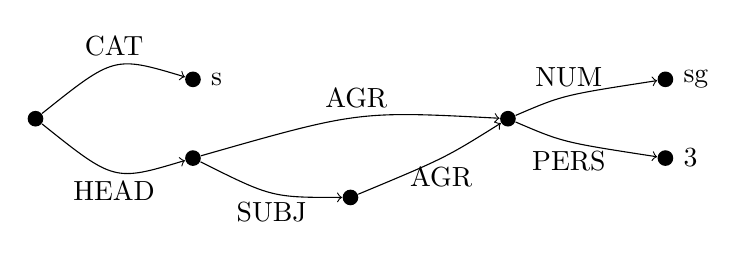
\begin{tikzpicture}
\tikzstyle{end} = [circle, minimum width=2pt, fill, inner sep=2pt]
\node [end] (n0) at (0,0) {};
\node [end, label=right: s] (n1) at (2, 0.5) {};
\node [end] (n2) at (2, -0.5) {};
\node [end] (n3) at (4,-1) {};
\node [end] (n4) at (6,0) {};
\node [end, label=right: sg] (n5) at (8,0.5) {};
\node [end, label=right: 3] (n6) at (8,-0.5) {};
\draw [->] (n0) .. controls (1,0.8) .. node [above] {CAT} (n1);
\draw [->] (n0) .. controls (1,-0.8) .. node [below] {HEAD} (n2);
\draw [->] (n2) .. controls (3,-1) .. node [below] {SUBJ} (n3);
\draw [->] (n2) .. controls (4.1, 0.1) .. node [above] {AGR} (n4);
\draw [->] (n3) .. controls (5.2,-0.5) .. node [below] {AGR} (n4);
\draw [->] (n4) .. controls (6.7,0.3) .. node [above] {NUM} (n5);
\draw [->] (n4) .. controls (6.7, -0.3) .. node [below] {PERS} (n6);
\end{tikzpicture}
\end{center}

Here, the paths $\langle \textsc{head},\ \textsc{agr}\rangle$ and $\langle \textsc{head},\ \textsc{subj},\ \textsc{agr}\rangle$ both lead to the same node, i.e., they lead to the same value and share that value. This property of feature structures that several features can share one value is called reentrancy. It is one of the reasons why feature structures are so useful for computational linguistics.

In attribute value matrices, reentrancy is is commonly expressed by coindexing the values which are shared. Written in the matrix notation the graph from above looks as follows. The boxed 1 indicates that the two features sequences leading to it share one value.
\[
\begin{bmatrix}
CAT & s \\
HEAD & 
\begin{bmatrix}
AGR & \fbox{1}
\begin{bmatrix}
NUM & sg \\
PERS & 3 
\end{bmatrix} \\
SUBJ & 
\begin{bmatrix}
AGR & \fbox{1}
\end{bmatrix}
\end{bmatrix}
\end{bmatrix}
\]

\subsection{Comparing Feature Structures: Subsumption}

We said above that feature structures are essentially sets of properties. Given two different sets of properties an obvious thing to do is to compare the information they contain. A particularly important concept for comparing two feature structures is subsumption.

A feature structure F1  subsumes ($\sqsubseteq$) another feature structure F2, iff all the information that is contained in F1  is also contained in F2.

The following two feature structures for instance subsume each other. 
The both contain exactly the same information, since the order in which the features are listed in the matrix is not important.
\[
\begin{bmatrix}
NUMBER & sg \\
PERSON & 3
\end{bmatrix} \quad 
\begin{bmatrix}
PERSON & 3 \\
NUMBER & sg
\end{bmatrix}
\]

More examples,
\[
\begin{bmatrix}
NUMBER & sg
\end{bmatrix}
\sqsubseteq
\begin{bmatrix}
PERSON & 3 \\
NUMBER & sg
\end{bmatrix}
\]
and
\[
\begin{bmatrix}
PERSON & 3 \\
NUMBER & sg
\end{bmatrix}
\not\sqsubseteq
\begin{bmatrix}
NUMBER & sg
\end{bmatrix}
\]

\[
\begin{bmatrix}
NUMBER & sg \\
GENDER & masc 
\end{bmatrix}
\not\sqsubseteq
\begin{bmatrix}
PERSON & 3 \\
NUMBER & sg
\end{bmatrix}
\]
and
\[
\begin{bmatrix}
PERSON & 3 \\
NUMBER & sg
\end{bmatrix}
\not\sqsubseteq
\begin{bmatrix}
NUMBER & sg \\
GENDER & masc 
\end{bmatrix}
\]

Notice that the subsumption relation between feature structures is somewhat similar to the subset relation between sets: Feature structure $F_1$  subsumes features structure $F_2$  iff all the information of $F_1$  is also in $F_2$. Set $S_1$  is a subset of set $S_2$  iff all elements of $S_1$  are also elements of $S_2$.

\subsection{Feature Structure Unification}

Unification ($\sqcup$) is a (partial) operation on feature structures. Intuitively, it is the operation of combining two feature structures such that the new feature structure contains all the information of the original two, and nothing more.

For example, 
\begin{align*}
F_1 &=
\begin{bmatrix}
CAT & np \\
AGREE & 
\begin{bmatrix}
NUMBER & singular
\end{bmatrix}
\end{bmatrix} \\
F_2 &= 
\begin{bmatrix}
CAT & np \\
AGREE &
\begin{bmatrix}
PERSON & third
\end{bmatrix}
\end{bmatrix} \\
F_1 \sqcup F_2 &=
\begin{bmatrix}
CAT & np \\
AGREE & 
\begin{bmatrix}
NUMBER & singular \\
PERSON & third
\end{bmatrix}
\end{bmatrix}
\end{align*}

Clearly $F_1\ \sqcup \ F_2$  contains all the information that is in $F_1$  and $F_2$  -- and it doesn't contain any other information. 

Why did we call unification a partial operation? Why didn't we just say that it was an operation on feature structures? The point is that unification is not guaranteed to return a result. For example, let 
\begin{align*}
F_3 &=
\begin{bmatrix}
CAT & np
\end{bmatrix} \\
F_4 &=
\begin{bmatrix}
CAT & vp
\end{bmatrix}
\end{align*}
Then $F_3\ \sqcup \ F_4$  does not exist. There is no feature structure that contains all the information in $F_3$  and $F_4$, because the information in these two feature structures is contradictory. So, the value of this unification is undefined.

The unification of two feature structures $F$  and $G$  (if it exists) is the smallest feature structure that is subsumed by both $F$  and $G$. That is, $F\ \sqcup \ G$  (if it exists) is the feature structure with the following three properties: 
\begin{enumerate*}
\item $F\ \sqsubseteq \ F\sqcup G$ ($F\ \sqcup \ G$ is subsumed by $F$)
\item $G\ \sqsubseteq \ F\sqcup G$ ($F\ \sqcup \ G$ is subsumed by $G$)
\item If $H$ is a feature structure such that $F\sqsubseteq H$ and $G\sqsubseteq H$, then $F\sqcup G \sqsubseteq \ H$ ( $F\ \sqcup \ G$ is the smallest feature structure fulfilling the first two properties. That is, there is other feature structure that also has properties 1 and 2 and subsumes $F\ \sqcup \ G$.)
\end{enumerate*}

If there is no smallest feature structure that is subsumed by both $F$  and $G$, then we say that the unification of $F$  and $G$ is undefined. 

We said above that the subsumption relation $\sqsubseteq$  on feature structures can be thought of as analogous to the subset relation on sets. Similarly, unification $\sqcup$  is rather like an analog of set-theoretic union (recall that the union of two sets is the smallest set that contains all the elements in both sets). But there is a difference: union of sets is an operation  (that is, the union of two sets is always defined) whereas (as we have discussed) unification is only a partial operation on feature structures.

More examples,
\begin{align*}
F_5 &= 
\begin{bmatrix}
AGREE & 
\begin{bmatrix}
NUMBER & singular
\end{bmatrix} \\
SUBJECT & 
\begin{bmatrix}
AGREE &
\begin{bmatrix}
NUMBER & singular
\end{bmatrix}
\end{bmatrix}
\end{bmatrix}\\
F_6 &=
\begin{bmatrix}
SUBJECT &
\begin{bmatrix}
AGREE &
\begin{bmatrix}
PERSON & third
\end{bmatrix}
\end{bmatrix}
\end{bmatrix}\\
F_5 \sqcup F_6 &=
\begin{bmatrix}
AGREE & 
\begin{bmatrix}
NUMBER & singular
\end{bmatrix} \\
SUBJECT &
\begin{bmatrix}
AGREE &
\begin{bmatrix}
NUMBER & singular \\
PERSON & third
\end{bmatrix}
\end{bmatrix}
\end{bmatrix}\\
F_7 &= 
\begin{bmatrix}
AGREE & \fbox{1}
\begin{bmatrix}
NUMBER & singular
\end{bmatrix} \\
SUBJECT &
\begin{bmatrix}
AGREE & \fbox{1}
\end{bmatrix}
\end{bmatrix} \\
F_6 \sqcup F_7 &=
\begin{bmatrix}
AGREE & \fbox{1}
\begin{bmatrix}
NUMBER & singular \\
PERSON & third
\end{bmatrix} \\
SUBJECT & 
\begin{bmatrix}
AGREE & \fbox{1}
\end{bmatrix}
\end{bmatrix}
\end{align*}
Specially,
\[
F \sqcup [\ ]=[\ ] \sqcup F=F
\]

\subsection{Generalization}

Generalization can be thought of as an analog of the set-theoretic operation of intersection. Recall that the intersection of two sets is the set that contains only the elements common to both sets. Similarly, the generalization of two feature structures contains only the information that is common to both feature structures. For example,
\begin{align*}
F_9 &= 
\begin{bmatrix}
AGREE & 
\begin{bmatrix}
NUMBER & plural \\
PERSON & third
\end{bmatrix} \\
ARITY & 3
\end{bmatrix} \\
F_{10} &=
\begin{bmatrix}
AGREE & 
\begin{bmatrix}
NUMBER & plural \\
PERSON & first
\end{bmatrix} \\
ARITY & 1
\end{bmatrix} \\
F_9 \sqcap F_{10} &= 
\begin{bmatrix}
AGREE & 
\begin{bmatrix}
NUMBER & plural
\end{bmatrix}
\end{bmatrix}
\end{align*}

Here's a precise definition of generalization: The generalization of two feature structures F  and G  is the largest feature structure that subsumes both F  and G. That is, $F\ \sqcap \ G$  is the feature structure with the following three properties: 
\begin{enumerate*}
\item $F\sqcap G\ \sqsubseteq \ F$
\item $F\sqcap G \ \sqsubseteq \ G$
\item If H is a feature structure such that $H\sqsubseteq F$ and $H\sqsubseteq G$, then $H\ \sqsubseteq \ F\sqcup G$
\end{enumerate*}

There is an important difference between unification and generalization: unlike unification, generalization is an operation on feature structures, not just a partial operation. That is, the generalization of two features is always defined. Think about it. Consider the worst case --- two feature structures F  and G  that contain no common information at all. Is there a largest feature structure that subsumes both? Of course there is --- the empty feature structure $[\ ]$. 

\subsection{合一算法的实现}

首先给出复杂特征集的数据结构。

约束的实现也可以不借用复杂特征集和合一运算来实现,可以有更直观的实现方法。约束有两大类型:1)只与规则中单个符号相关;2)涉及到多个符号。前者的表现形式是二元组:属性名-属性值,后者表示成IF语句的形式。合一算法与图分析方法结合。每个edge都带有一个属性约束集合,随着edge的生长,属性约束结合也不断地实例化和变化,有时会判断edge是不合适的,中断这个edge的生长。

\section{分析算法的实现}

先看一种常规的实现方法。这种方法规则是顺序存放在数组中,每次查询规则都要顺序扫描一趟数组,效率较低。改进的方法是用树结构存放规则。

\begin{verbatim}
class ruleitemclass {
  int ruleid;
  int ruleloc;
}

class sentlocclass {
  int start;
  int end;
}

class edgeclass {
  public:
  ruleitemclass ruleitem;
  sentlocclass sentloc;

  bool operator<(edgeclass const& other) const {
    if (sentloc != other.sentloc) {
      return(sentloc < other.sentloc)
    }
    else if (ruleitem != other.ruleitem) {
      return (ruleitem < other.ruleitem);
    }
    else {
      return(0);
    }
  }
}

set<edgeclass> chart;
queue<edgeclass> agenda;

void forward(edgeclass *edgep)
{
 for (set<edgeclass>::iterator i=chart.begin(); i!=chart.end(); i++) {
   if ( (i->sentloc.start == edgep->sentloc.end) &&
        (ruleset[i->ruleid].reduct == ruleset[edgep->ruleid].forest[edgep->ruleloc]) &&
        (
 } 
}
\end{verbatim}

\section{属性约束的分析}

分析的主要目的是,发现约束中对应的短语。

\begin{figure}
  \begin{center}
    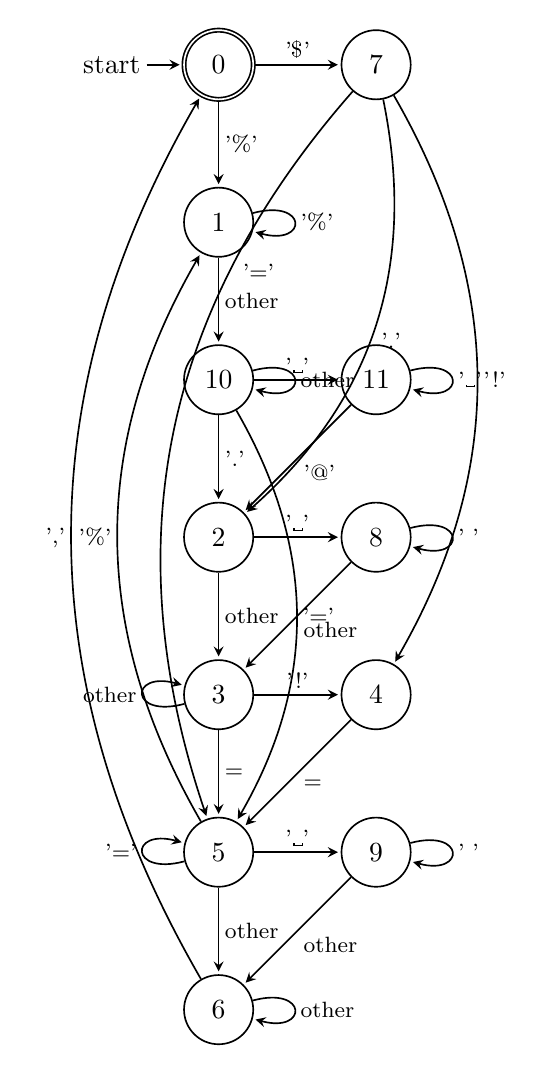
\begin{tikzpicture}[->, >=stealth, shorten >=1pt, auto, node distance=2cm, semithick, inner sep=2pt, bend angle=30]
      
      \node[initial, accepting, state] (s0) {0};
      \node[state] (s1) [below of=s0] {1};
      \node[state] (s10) [below of=s1] {10};
      \node[state] (s11) [right of=s10] {11};
      \node[state] (s2) [below of=s10] {2};
      \node[state] (s3) [below of=s2] {3};
      \node[state] (s4) [right of=s3] {4};
      \node[state] (s5) [below of=s3] {5};
      \node[state] (s6) [below of=s5] {6};
      \node[state] (s7) [right of=s0] {7};
      \node[state] (s8) [right of=s2] {8};
      \node[state] (s9) [right of=s5] {9};
      
      \tikzstyle{every node}=[font=\footnotesize]
      \path 
      (s0) edge node {'\%'} (s1)
      (s0) edge node {'\$'} (s7)
      (s1) edge [loop right] node {'\%'} (s1)
      (s1) edge node {other} (s10)
      (s10) edge [loop right] node {other} (s10)
      (s10) edge node {'.'} (s2)
      (s2) edge node {other} (s3)
      (s2) edge node {'\textvisiblespace'} (s8)
      (s8) edge node {other} (s3)
      (s3) edge node {'!'} (s4)
      (s3) edge node {=} (s5)
      (s3) edge [loop left] node {other} (s3)
      (s4) edge node {=} (s5)
      (s5) edge node {other} (s6)
      (s6) edge [loop right] node {other} (s6)
      (s5) edge [bend left] node {'\%'} (s1)
      (s5) edge node {'\textvisiblespace'} (s9)
      (s9) edge node {other} (s6)
      (s6) edge [bend left] node {','} (s0)
      (s7) edge [bend left] node {'.'} (s2)
      (s8) edge [loop right] node {' '} (s8)
      (s9) edge [loop right] node {' '} (s9)
      (s7) edge [bend left] node {'!'} (s4)
      (s7) edge [bend right] node [near start] {'='} (s5)
      (s10) edge node {'\textvisiblespace'} (s11)
      (s11) edge [loop right] node {'\textvisiblespace'} (s11)
      (s11) edge node {'@'} (s2)
      (s10) edge [bend left] node {'='} (s5)
      (s5) edge [loop left] node {'='} (s5);
    \end{tikzpicture}
    \caption{属性约束等式的分析}
    \label{fig:equbind}
  \end{center}
\end{figure}

一点问题。如下的文法可能出现IF语句中的嵌套,这是不合理的。
\begin{verbatim}
<Bind>:
       <Equation>
       <Test>
       <Bind> , <Bind>
<Test>:
       IF <Bind> TRUE
       IF <Bind> FALSE
       IF <Bind> THEN <Bind> ENDIF
       IF <Bind> ELSE <Bind> ENDIF
       IF <Bind> THEN <Bind> ELSE <Bind> ENDIF
\end{verbatim}

比如出现如下约束,这是难以理解的。
\begin{verbatim}
 <BIND> -> <Test> 
        -> IF <Bind> TRUE
        -> IF <Test> TRUE
        -> IF IF <Bind> FALSE TRUE
        -> IF IF <Equation> FALSE TRUE
\end{verbatim}

利用逗号拆分各个约束的状态图。

\begin{figure}
  \begin{center}
    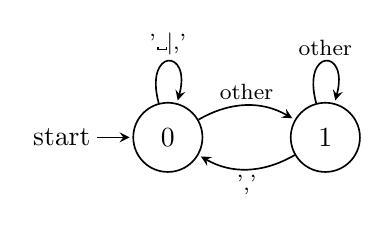
\begin{tikzpicture}[->, >=stealth, shorten >=1pt, auto, node distance=2cm, semithick, inner sep=2pt, bend angle=30]
      
      \node[initial, state] (s0) {0};
      \node[state] (s1) [right of=s0] {1};
      
      \tikzstyle{every node}=[font=\footnotesize]
      \path 
      (s0) edge [loop above] node {'\textvisiblespace$|$,'} (s0)
      (s0) edge [bend left] node {other} (s1)
      (s1) edge [loop above] node {other} (s1)
      (s1) edge [bend left] node {','} (s0);
    \end{tikzpicture}
    \caption{利用逗号拆分约束的状态图}
    \label{fig:puncbind}
  \end{center}
\end{figure}

现在属性约束中的所有语法类别都用数字(即它在规则中的位置)替代了,我们还需要找出这个数字来。再次利用图\ref{fig:equbind},稍作修改得到图\ref{fig:permbind},利用它来完成属性约束的演算(将来可以考虑将这两个处理合二为一)。

\begin{figure}
  \begin{center}
    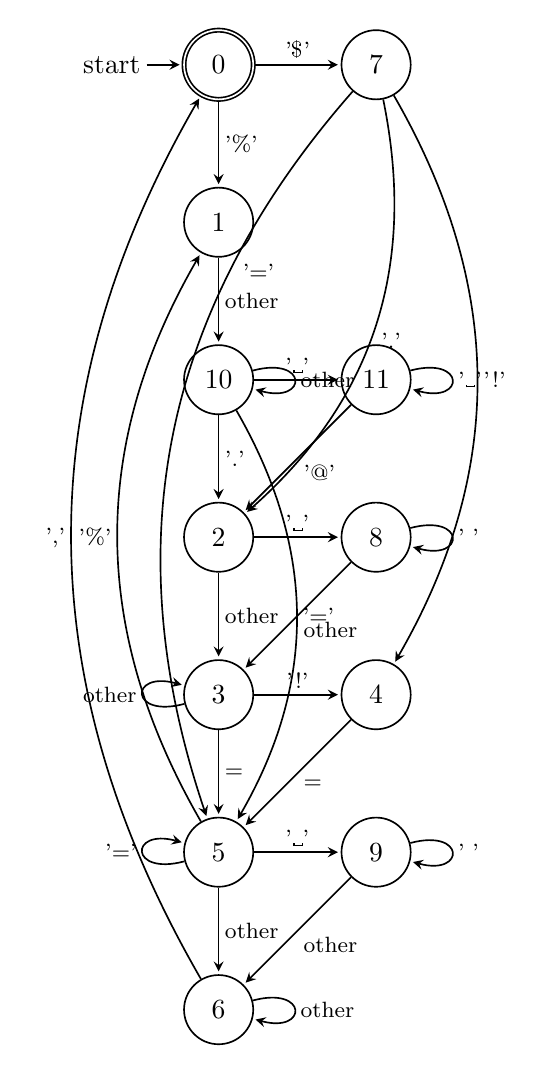
\begin{tikzpicture}[->, >=stealth, shorten >=1pt, auto, node distance=2cm, semithick, inner sep=2pt, bend angle=30]
      
      \node[initial, accepting, state] (s0) {0};
      \node[state] (s1) [below of=s0] {1};
      \node[state] (s10) [below of=s1] {10};
      \node[state] (s11) [right of=s10] {11};
      \node[state] (s2) [below of=s10] {2};
      \node[state] (s3) [below of=s2] {3};
      \node[state] (s4) [right of=s3] {4};
      \node[state] (s5) [below of=s3] {5};
      \node[state] (s6) [below of=s5] {6};
      \node[state] (s7) [right of=s0] {7};
      \node[state] (s8) [right of=s2] {8};
      \node[state] (s9) [right of=s5] {9};
      
      \tikzstyle{every node}=[font=\footnotesize]
      \path 
      (s0) edge node {'\%'} (s1)
      (s0) edge node {'\$'} (s7)
      (s1) edge node {other} (s10)
      (s10) edge [loop right] node {other} (s10)
      (s10) edge node {'.'} (s2)
      (s2) edge node {other} (s3)
      (s2) edge node {'\textvisiblespace'} (s8)
      (s8) edge node {other} (s3)
      (s3) edge node {'!'} (s4)
      (s3) edge node {=} (s5)
      (s3) edge [loop left] node {other} (s3)
      (s4) edge node {=} (s5)
      (s5) edge node {other} (s6)
      (s6) edge [loop right] node {other} (s6)
      (s5) edge [bend left] node {'\%'} (s1)
      (s5) edge node {'\textvisiblespace'} (s9)
      (s9) edge node {other} (s6)
      (s6) edge [bend left] node {','} (s0)
      (s7) edge [bend left] node {'.'} (s2)
      (s8) edge [loop right] node {' '} (s8)
      (s9) edge [loop right] node {' '} (s9)
      (s7) edge [bend left] node {'!'} (s4)
      (s7) edge [bend right] node [near start] {'='} (s5)
      (s10) edge node {'\textvisiblespace'} (s11)
      (s11) edge [loop right] node {'\textvisiblespace'} (s11)
      (s11) edge node {'@'} (s2)
      (s10) edge [bend left] node {'='} (s5)
      (s5) edge [loop left] node {'='} (s5);
    \end{tikzpicture}
    \caption{属性约束等式的演算}
    \label{fig:permbind}
  \end{center}
\end{figure}

\newpage
\appendix
\section{刘群给出的词法和文法总结}

在本说明中,括在尖括号中的部分,如 \verb|<Ident>|,表示 Ident 是本说明中用到的概念。而尖括号中如果出现冒号,如 \verb|<Ident:LexCat>|,则表示 LexCat 是对概念 Ident的一些限定。

以下例子介绍本文在说明一个概念时所采用的形式:

\vspace{1pc}
\begin{verbatim}
<PhrAtt>:
        PhrAtt : { <Att_Set> }
        PhrAtt <Condition> : { <Att_Set> }
\end{verbatim}

在这个例子中,第一行表示被说明的概念是\verb|<PhrAtt>|,后面两行表示这个概念有两种形式。后面两行中又用到了关键字 \verb|PhrAtt|, \verb|PhrCat|, 分隔符 \verb|( ) { }| : , 和其它几个概念:\verb|<Attribute>|, \verb|<Att_Set>|, 和 \verb|<Condition>|。

\begin{verbatim}

§0  数据文件的词法

        关键字:

                SemModel        SynModel        EndModel
                SemCat          SemAtt          SemVal
                LexCat          LexAtt          LexVal
                PhrCat          PhrAtt          PhrVal
                SemAssAtt       SemAssVal       SynAssAtt       SynAssVal
                BaseForm        VaryForm        Static          Dynamic
                Limited         Unlimited       RelMode         Default
                Hierar          Symbol          Number          Boolean
                Field           Digit           Punct           Other
                IF              TRUE            FALSE
                THEN            ELSE            ENDIF

        标识符:

        <Ident>:
                <NrmIdent>
                <StrIdent>
        <NrmIdent>:
                <Alpha>
                <NrmIdent><Alpha>
                <NrmIdent><Digit>
        <StrIdent>:
                "<String>"
        <Alpha>:
                _
                <ChnChar>
                <LtnChar>
        <LtnChar>:
                A-Z
                a-z
        <ChnChar>:
                汉字
        <Digit>:
                0-9
        <String>:
                任意字符串, 其中的双引号(")重复一次

        数:

        <Integ>:
                <Digit>
                <Integ><Digit>

        分隔符:

                . , ; : = | ~ ~~
                ( ) < > [ ] { }
                ^ && ## $$ ** ! $ / & * + -> => == != :: << >>  -- ||
                % %% %%% %%%%
                / // /// ////

        注释:

          位于 /* 和 */ 之间的字符串

        语言代码:

        <LangCode>:
                CHINESE
                ENGLISH

        除了以字母(包括汉字和下横线)开头的字母数字串以外,括在双引号中的任意字符
串也可以作为标识符使用,用于表示标点符号等特殊符号。双引号内的字符串中如果又
出现双引号(")应重复一次, 用两个双引号("")表示。 除非在双引号内,否则标识符中
不允许出现空白符号。两个标识符之间必须有空白或其它符号分隔。

§1  语言模型

<Model>:
        <SemModel>
        <Model> <SynModel>
<SemModel>:
        SemModel <SemModelBody> EndModel
<SemModelBody>:
        <SemCat> <SemFeat> <SemAss>
<SynModel>:
        SynModel ( <LangCode> ) <SynModelBody> EndModel
<SynModelBody>:
        <LexCat> <LexFeat> <PhrCat> <PhrFeat> <SynAss> <SpecialField>

<SemCat>:
        SemCat : <Attribute> : { <HieSym_Set> }

<SemFeat>:
        <SemAtt>
        <SemVal>
        <SemFeat> <SemFeat>

<SemAtt>:
        SemAtt : { <Att_Set> }
        SemAtt <Condition> : { <Att_Set> }

<SemVal>:
        SemVal ( <Ident:SemAtt> ) : <AtomVal>

<Condition>:
        <Fest>

<AtomVal>:
        <AtomValType>
        <AtomValType> <ValMode>
<AtomValType>:
        <AtomType>
        <AtomType> <DefAtom>
<ValMode>:
        <ActMode>
        <RelMode>
        <ActMode> <RelMode>
<DefAtom>:
        Default = <Atom>
<ActMode>:
        Static
        Dynamic
<RelMode>:
        RelMode = 0
        RelMode = 1

<Att_Set>:
        <Attribute>
        <Att_Set> , <Attribute>
<Attribute>:
        <Att_Name>
        <Attribute> = <Att_Alias>
<Att_Name>:
        <Ident>
<Att_Alias>:
        <Ident>

<AtomType>:
        Hierar Unlimited
        Hierar Unlimited { <HieSym_Set> }
        Hierar Limited   { <HieSym_Set> }
        Symbol Unlimited
        Symbol Unlimited { <HieSym_Set> }
        Symbol Limited   { <HieSym_Set> }
        Number Unlimited
        Number Unlimited { <Number_Set> }
        Number Limited   { <Number_Set> }
        Boolean
        Boolean { <Boolean_Set> }
<HieSym_Set>:
        <HieSym_Atom>
        <HieSym_Set> , <HieSym_Atom>
<HieSym_Atom>:
        <Atom_Name>
        <HieSym_Atom> = <Atom_Alias>
<Atom_Name>:
        <Ident>
<Atom_Alias>:
        <Ident>
<Number_Set>:
        <Number_Atom>
        <Number_Set> , <Number_Atom>
<Number_Atom>:
        <Integ> = <Atom_Alias>
        <Number_Atom> = <Atom_Alias>
<Boolean_Set>:
        <Boolean_Atom>
        <Boolean_Set> , <Boolean_Atom>
<Boolean_Atom>:
        <True> = <Atom_Alias>
        <False> = <Atom_Alias>
        <Boolean_Atom> = <Atom_Alias>
<True>:
        是
        Yes
        YES
<False>:
        否
        No
        NO

<SemAss>:
        <SemAssAtt>
        <SemAssVal>
        <SemAss> <SemAss>
<SemAssAtt>:
        SemAssAtt : { <Att_Set> }
        SemAssAtt <Condition> : { <Att_Set> }
<SemAssVal>:
        SemAssVal ( <Ident:SemAssAtt> ) : <FestVal>
<FestVal>:
        <DefFest>
        <ValMode>
        <DefFest> <ValMode>
<DefFest>:
        Default = <Fest>

<LexCat>:
        LexCat : <Attribute> : { <HieSym_Set> }

<LexFeat>:
        <LexAtt>
        <LexVal>
        <LexFeat> <LexFeat>

<LexAtt>:
        LexAtt ( BaseForm ) : <Attribute>
        LexAtt ( VaryForm ) : <Attribute>
        LexAtt : { <Att_Set> }
        LexAtt <Condition> : { <Att_Set> }

<LexVal>:
        LexVal ( <Ident:LexAtt> ) : <AtomVal>

<PhrCat>:
        PhrCat : <Attribute> : { <HieSym_Set> }

<PhrFeat>:
        <PhrAtt>
        <PhrVal>
        <PhrFeat> <PhrFeat>

<PhrAtt>:
        PhrAtt : { <Att_Set> }
        PhrAtt <Condition> : { <Att_Set> }

<PhrVal>:
        PhrVal ( <Ident:PhrAtt> ) : <AtomVal>

<SynAss>:
        <SynAssAtt>
        <SynAssVal>
        <SynAss> <SynAss>
<SynAssAtt>:
        SynAssAtt : { <Att_Set> }
        SynAssAtt <Condition> : { <Att_Set> }
<SynAssVal>:
        SynAssVal ( <Ident:SynAssAtt> ) : <FestVal>

<SpecialField>:
        <DigitField> <PunctField> <OtherField>
<DigitField>:
        Field ( Digit ) : <Ident:LexCat>
        Field ( Digit ) : <Ident:LexCat> <Fest>
<PunctField>:
        Field ( Punct ) : <Ident:LexCat>
        Field ( Punct ) : <Ident:LexCat> <Fest>
<OtherField>:
        Field ( Other ) : <Ident:LexCat>
        Field ( Other ) : <Ident:LexCat> <Fest>

§2  描述语言知识的基本形式

<Atom>:
        <Hierar>
        <Symbol>
        <Number>
        <Boolean>
<Hierar>:
        <Hierar_Or>
<Hierar_Or>:
        <Hierar_And>
        <Hierar_Not>
        <Hierar_Or>|<Hierar_And>
<Hierar_And>:
        <Hierar_Smp>
        <Hierar_And>~<Hierar_Smp>
<Hierar_Not>:
        ~<Hierar_Smp>
        <Hierar_Not>~<Hierar_Smp>
<Hierar_Smp>:
        <Ident:Atom_Name>
        <Ident:Atom_Alias>
<Symbol>:
        <Symbol_Or>
        <Symbol_Not>
<Symbol_Or>:
        <Symbol_Smp>
        <Symbol_Or>|<Symbol_Smp>
<Symbol_Not>:
        ~<Symbol_Smp>
        <Symbol_Not>~<Symbol_Smp>
<Symbol_Smp>:
        <Ident:Atom_Name>
        <Ident:Atom_Alias>
<Number>:
        <Number_Or>
        <Number_Not>
<Number_Or>:
        <Number_Smp>
        <Number_Or>|<Number_Smp>
<Number_Not>:
        ~<Number_Smp>
        <Number_Not>~<Number_Smp>
<Number_Smp>:
        <Integ>
        <Ident:Atom_Alias>
<Boolean>:
        <True>
        <False>
        <Ident:Atom_Alias>

<Fest>:
        [ ]
        { }
        [ ] { }
        [ <IntFest> ]
        { <ExtFest> }
        [ <IntFest> ] { <ExtFest> }
        <None>
<IntFest>:
        <IntFeat>
        <IntFest> , <IntFeat>
        <IntFest> ; <IntFest>
<ExtFest>:
        <ExtFeat>
        <ExtFest> , <ExtFeat>
<IntFeat>:
        <IntAtt> : <IntVal>
<ExtFeat>:
        <ExtAtt> : <ExtVal>
<IntAtt>:
        <Ident:LexAtt>
        <Ident:PhrAtt>
        <Ident:SemAtt>
<ExtAtt>:
        <Ident:SemAss>
<IntVal>:
        <Atom>
<ExtVal>:
        <Fest>
<None>:
        无
        None
        NONE

<LeftForest>:
        <LeftTree>
        <HeadTag> <LeftTree>
        <LeftForest> <LeftForest>
<LeftTree>:
        <LabelItem>
        <LabelItem> < <WordItem_Or> >
        <LabelItem> ( <LeftSubForest> )
<LeftSubForest>:
        <LeftSubTree>
        <HeadTag> <LeftSubTree>
        <LeftSubForest> <LeftSubForest>
<LeftSubTree>:
        <LeftLabelItem>
        <LeftLabelItem> < <WordItem_Or> >
        <LeftLabelItem> ( <LeftSubForest> )
<LeftLabelItem>:
        <LabelItem>
<LabelItem>:
        <Ident:LexCat>
        <Ident:PhrCat>
<WordItem_Or>:
        <WordItem>
        <WordItem_Or> | <WordItem>
<WordItem>:
        ~~
        <Word>
<Word>:
        <Ident>
<HeadTag>:
        !

<RightForest>:
        <RightTree>
        <HeadTag> <RightTree>
        <RightForest> <RightForest>
<RightTree>:
        <LabelItem>
        <LabelItem> < <WordItem_Or> >
        <LabelItem> ( <LeftSubForest> )
<RightSubForest>:
        <RightSubTree>
        <HeadTag> <RightSubTree>
        <MoveTag> <ShiftLabelItem>
        <RemvTag> <ShiftLabelItem>
        <CopyTag> <ShiftLabelItem>
        <SubForest> <RightSubForest>
<RightSubTree>:
        <RightLabelItem>
        <RightLabelItem> < <WordItem_Or> >
        <RightLabelItem> ( <RightSubForest> )
<RightLabelItem>:
        <LabelItem>
        <LabelItem> <TransVar>
<ShiftLabelItem>:
        <LabelItem> <LabelVar>
<MoveTag>:
        #
<RemvTag>:
        &
<CopyTag>:
        *
<LabelVar>:
        <LabelVarTag> <LabelItem>
<TransVar>:
        <TransVarTag> <LabelItem>
<LabelVarTag>:
        %
        %%
        %%%
        %%%%
<TransVarTag>:
        /
        //
        ///
        ////

<Bind>:
        <Equation>
        <Test>
        <Bind> , <Bind>
<Test>:
        IF <Bind> TRUE
        IF <Bind> FALSE
        IF <Bind> THEN <Bind> ENDIF
        IF <Bind> ELSE <Bind> ENDIF
        IF <Bind> THEN <Bind> ELSE <Bind> ENDIF
<Equation>:
        <IntVar> = <Atom>
        <IntVar> = <IntVar>
        <ExtVar> = <Fest>
        <ExtVar> = <ExtVar>
        <ExtVar> = <True>
        <ExtVar> = <False>
        <ExtVar> == <ExtVar> <At>
        <ExtVar> != <ExtVar> <At>
<ExtVar>:
        <RootVar>
        <LabelVar>
        <ExtVar>.<ExtAtt>
<IntVar>:
        <ExtVar>.<IntAtt>
<RootVar>:
        $
<At>:
        @ <Ident:IntAtt>
        @ <Ident:ExtAtt>
        <At> <At>

§3  析句规则

<PrsRule>:
        && { <Title> } <PrsStruct> || <TrnSwitch> => <TrnStruct>
        && { <Title> } <PrsStruct> => <TrnStruct>
        <PrsRule> || <TrnSwitch> => <TrnStruct>
        <PrsRule> => <TrnStruct>
<Title>:
        <Ident>
        <Ident> / <Note>
<Note>:
        <Ident>
        <Note> <Ident>
        <Note> , <Ident>
<PrsStruct>:
        <PrsReductn> -> <PrsForest>
        <PrsReductn> -> <PrsForest> :: <PrsBind>
<PrsReductn>:
        <LabelItem>
<PrsForest>:
        <LeftForest>
        ^ <LeftForest>
<PrsBind>:
        <Bind>
<TrnSwitch>:
        <Bind>
<TrnStruct>:
        <TrnTree>
        <TrnTree> <TrnBind>
<TrnTree>:
        <RightTree>
<TrnBind>:
        <Bind>

§4  造句规则

<MakRule>:
        ## { <Title> } <LMakStruct> => <RMakStruct>
        <MakRule> => <RMakStruct>
<LMakStruct>:
        <LMakTree>
        <LMakTree> <LMakBind>
<LMakTree>:
        <LeftTree>
<LMakBind>:
        <Bind>
<RMakStruct>:
        <RMakTree>
        <RMakTree> <RMakBind>
<RMakTree>:
        <RightTree>
<RMakBind>:
        <Bind>

§5  词典

<Entry>:
        $$ <Word> <Meaning>
        <Entry> <Meaning>
        <Entry> <PrsRule>
<Meaning>:
        ** { <Title> } <SrcMeaning>
        <Meaning> || <TrnSwitch> => <TgtMeaning>
        <Meaning> => <TgtMeaning>
<SrcMeaning>:
        <LabelItem>
        <LabelItem> <Bind>
<TgtMeaning>:
        <TrnStruct>

§6  汉语切词规则

<CutRule>:
        @@ <CutLexVaryStruct> << <CutLexBaseStruct>
<CutLexVaryStruct>:
        <CutLexVary> -- <CutLexStruct>
<CutLexBaseStruct>:
        <CutLexBase> -- <CutLexStruct>
<CutLexStruct>:
        <LabelItem>
        <LabelItem> <Fest>
<CutLexVary>:
        <ChnChar>
        <CutCharVar>
        <CutLexVary> <CutLexVary>
<CutCharVar>:
        A-Z
<CutLexBase>:
        <ChnChar>
        <CutCharVar>
        <CutLexBase> <CutLexBase>

§7  汉语切分规则

<SegRule>:
        @@ <Word>

§8  英语构词规则

<BldRule>:
        @@ <BldLexBaseStruct> >> <BldLexVaryStruct>
<BldLexBaseStruct>:
        <BldLexBase> -- <BldLexStruct>
<BldLexVaryStruct>:
        <BldLexVary>
        { <Ident:LexAtt> }
<BldLexStruct>:
        <LabelItem>
        <LabelItem> <Fest>
<BldLexBase>:
        <LtnChar>
        <BldWordVar>
        <BldLexBase> <LtnChar>
<BldWordVar>:
        *
<BldLexVary>:
        <LtnChar>
        <BldWordVar>
        <BldLexVary> <LtnChar>
\end{verbatim}

\bibliographystyle{/media/3AA47D84A47D4403/txp/writing/paper/share/chinesebst}
\bibliography{/media/3AA47D84A47D4403/txp/writing/paper/share/tao-cl-doc}

\end{CJK}
\end{document}
